\documentclass[11pt]{article}

\usepackage{common}
\usepackage{booktabs}
\usepackage[margin=1in]{geometry}
\usepackage{hyperref}
\title{The Analytics Edge, Final Report:\\ Building a Topic Model as a First Step Toward an Article Recommender for Bleacher Report Basketball}
\author{for Professor Dimitris Bertsimas and Emma Gibson \text{ } \\ \\ by Stephen Albro \& Cyrille Combettes \\ salbro@mit.edu, cyrille@mit.edu}
\begin{document}
\maketitle{}


\section{Motivation and Project Abstract}
Websites need to retain visitors to compete for advertising revenue. Bleacher Report, a primary online destination for sports readers, competes for an audience with ESPN.com and others. Bleacher Report has a two-fold hope for each visitor. First, \textit{prolonged} visits: that the visitor spends a lot of time on the website, jumping from article to article.  Second, \textit{frequent} visits: that the visitor develops loyalty to the website.  We feel that having a micro-targeted article recommendation system would help Bleacher Report foster long visits and loyalty among its readers, providing an analytics-based edge over its competitors.  As basketball fans, we developed a strong first step toward a basketball article recommender system.

A reasonable way to build an article recommender is to \textit{embedding} each article in some meaningful vector space, and then, using visitor's history, recommend nearest neighbors within that space. This project focuses on exploring an article-embedding strategy based on \textit{topics} found in the articles. This strategy is known as \textit{topic modeling}, and approach we chose is \textit{Latent Dirichlet Allocation (LDA)}.  

We briefly note that we determined LDA to be the most promising from among three article-embedding approaches by conducting an initial experiment, which  can be found in the appendix. We tested two other approaches: word2vec title embeddings, and Non-Negative Matrix Factorization topic modeling. 

\section{Data Collection}
Bleacher Report does not provide database access to articles.  However, NewsAPI is a company that provides access to news metadata, including URLs, from a variety of sources including Bleacher Report.  We queried NewsAPI for Bleacher Report articles from the start of the 2017-2018 NBA season. Our entire query consisted of joining the terms \textit{basketball} and \textit{NBA} with all 30 teams and the top 25 players.  We then scraped all 3314 URLs to obtain the articles.

\section{Data Cleaning}
Real-world data is never clean, but text data is particularly messy. Much preprocessing was necessary to prepare the articles for analysis. We made cleaning decisions with topic modeling in mind.  In particular, a bag-of-words cleaning approach was chosen over one that preserved grammar.

First, we \textit{tokenized} each article. In natural language processing, tokenizing means chopping a document into pieces, the most common way being to tokenize by \textit{word}. This is what we did.  We discarded non-alphabetical tokens (e.g. 8pm, 704, !, .) and converted everything to lower case.  Then, we removed 170 basic \textit{stop-words}, such as \textit{a, the, his}, and \textit{my}. 

Next, we needed to create custom tokens for players, teams, and coaches, since each player can be referred to in a variety of ways. For example, the NBA superstar LeBron James can also be called LeBron, Bron, or James.  We replaced all forms of each entity with a full, underscored version, so that, for example, every form of the above superstar would be converted to lebron\_james.  At times it was necessary to \textit{infer} the meaning of a word from ambiguous usage. For example, we concluded that the word \textit{Boston} should be replaced by boston\_celtics only if the entire phrase Boston Celtics appeared somewhere else in the article.  This application-specific tokenization allowed us to capture more contextual information about each superstar, team, and coach.

Next, we \textit{stemmed} each word. Stemming addresses the fact that the root of a word (e.g. \textit{play}) can take different grammatical forms (\textit{playing, played, plays}). A stemming simplification makes sense for topic modeling.

Finally, we reduced our vocabulary. In NLP, a \textit{vocabulary} is the complete set of words fed into a model.  As topic modelers, we wanted to preserve information-containing words (player and team tokens, high-impact verbs, league terminology), and remove mundane words from our articles.

We used \textit{document frequency} to help us choose the vocabulary. The document frequency of a word is the fraction of articles in which the word appears. The word \textit{the} has a document frequency of 1.0 (this is already a stop word). If a word occurs too \textit{infrequently}, it is probably an article-specific entity, and is thus unhelpful from a topical standpoint. On the other hand, if a word occurs too \textit{frequently}, it is probably a common word and  contains equally little topical information.

Therefore we sought lower and upper document-frequency cutoff thresholds to narrow our vocabulary.  We knew the upper threshold had to be at least as high as the document frequency of LeBron James at 0.22, since he is the most famous player and the vocabulary needs to include every player. After eye-test experimentation we decided upon an upper threshold 0.23. Our lower threshold was 0.01, discarding words appearing in less than 34 out of 3314 articles.  The words with within the range (0.01, 0.23) numbered about 3500 in all.
% REMOVED: After seeing irrelevant words persist with even an upper threshold of 0.5, we knew that the upper threshold had to be lower than that. 

\section{Topic Modeling with Latent Dirichlet Allocation}
In this section we introduce and discuss the training and tuning of our LDA topic model, which again, will help us discover topics with the goal of embedding articles in topic space for neighbor-based recommendation. We explore our results with insightful visualizations of the Bleacher Report topic landscape, and then do a final sanity-check of our model's topics by clustering articles in topic space.

\subsection{Introduction to Topic Modeling and LDA}
We introduce topic modeling and LDA more thoroughly in the appendix, but let us mention a few things.

Topic modeling aims to discover $k$ \textit{topics} from among a set of articles, and to estimate the proportion of each topic in each article.  A \textit{topic} is defined as a frequency distribution over all words in the vocabulary: for each topic, each word has a frequency of occurrence.  If topic modeling is successful, the high-frequency words for each topic will frequently appear together in text and will resemble the human understanding of a topic. 

Latent Dirichlet Allocation (LDA) is a type of topic model that assumes a generative story about the data.  We provide $k$, the number of topics, and LDA infers the latent topic-word distributions and article-topic distributions by using maximum likelihood estimation according to the generative story.  LDA's name comes from sparse Dirichlet priors that it employs: each document is assumed to come from only a small set of topics, and each topic is assumed to cover only a small set of words.

In the end, the fitted model allows us to achieve our goal of embedding each article as a vector, namely a distribution over all $k$ topics which represents its estimated topical proportions. The vector-embedded articles can then be used for nearest-neighbor recommendation. 

\subsection{Training LDA with Grid Search}
When training the LDA model in Python, we fine-tuned two hyper-parameters using grid-search cross-validation. The first was $k$, the number of topics.  The second was $\gamma$, the solver's learning rate.  Since topic modeling is an unsupervised problem, there was no need for a separate validation set, nor was there a supervising variable.  Instead, we used the log-likelihood of the trained model as our measure of model quality. 

First, we searched $k \in \{10, 15, 20, 25, 30\}$ and $\gamma \in \{.5, .7, .9\}$. On the left we plot the log-likelihoods for each parameter duo. After discovering finding an optimal $k=10$ and $\gamma = 0.7$, we narrowed the grid search (right) to find the absolute best $k$.  After searching $k \in \{10, 11, 12, 13, 14\}$ and $\gamma \in \{.5, .7, .9\}$, we found the optimal $k=13$ topics and $\gamma = 0.7$. \\

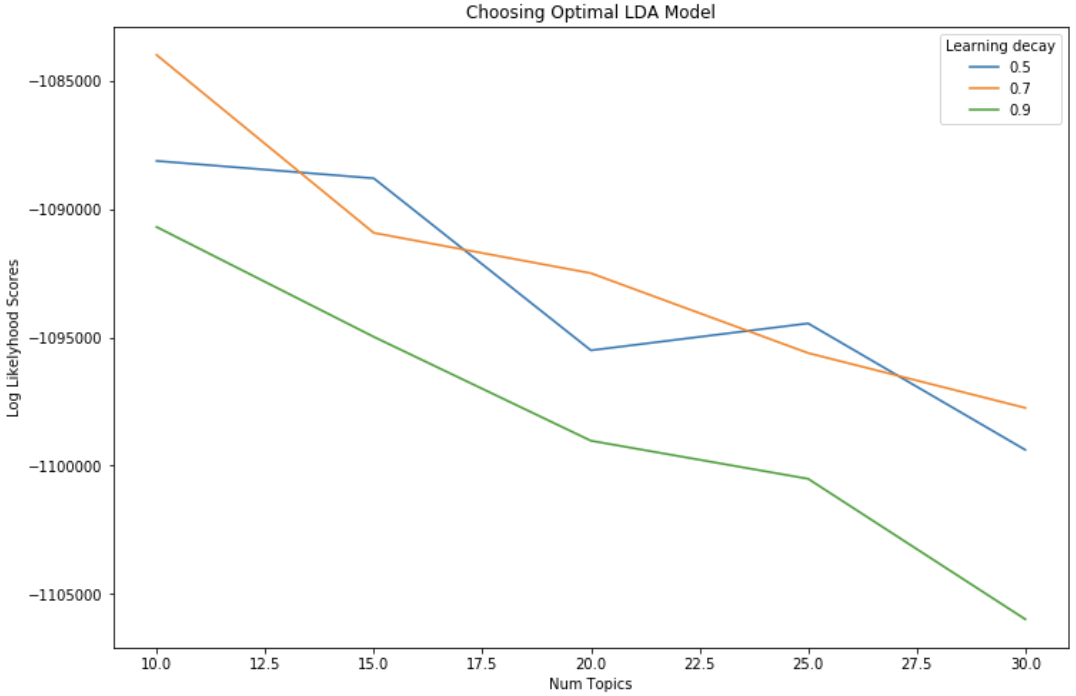
\includegraphics[width=225pt]{gridsearch.png} 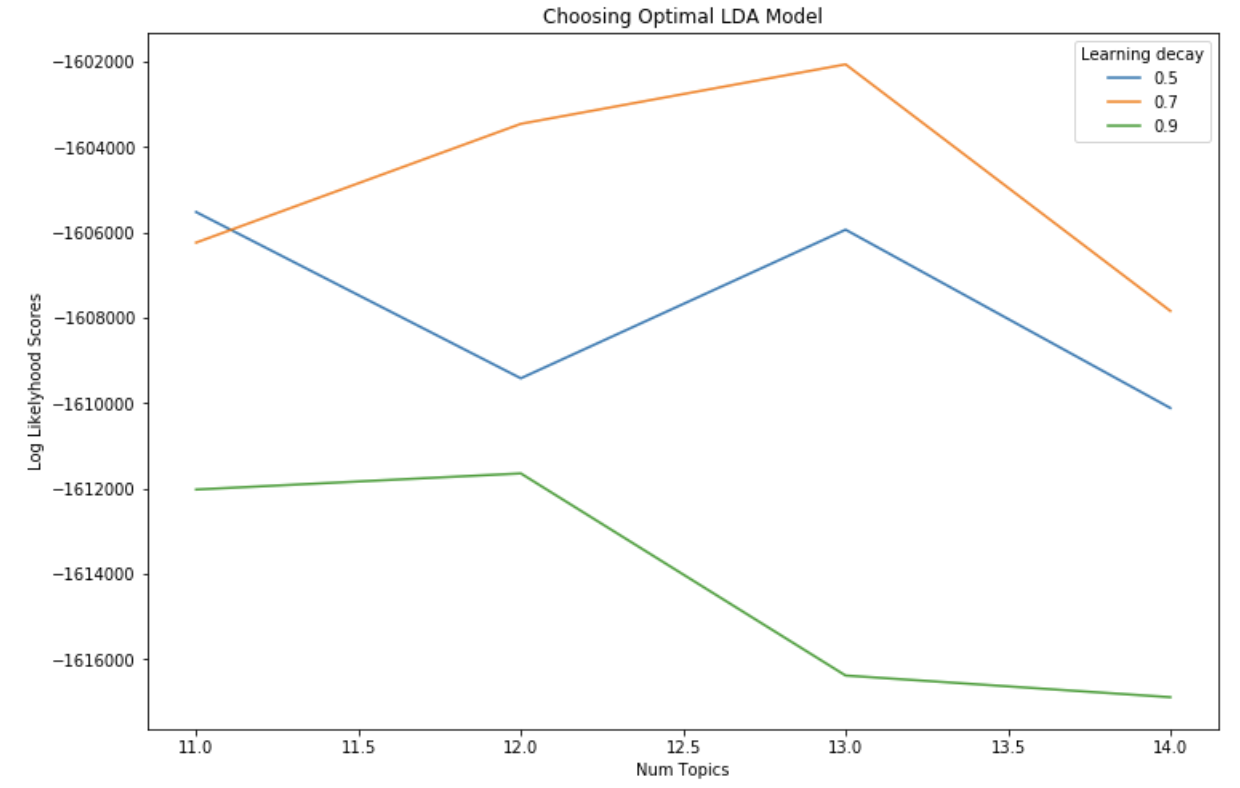
\includegraphics[width=225pt]{gridsearch2.png} 

\subsection{LDA Results}
\subsubsection{Visualization}
As avid NBA fans, we were pleased to discover that our topics made sense.  We visualized them using LDAvis, a method developed by Carson Siever and Kenneth Shirley \footnote{Sievert, Carson and Shirley, Kenneth. "LDAvis: A method for visualizing and interpreting topics". \textit{Proceedings of the Workshop of Interactive Language Learning, Visualization, and Interfaces}, pages 63-70, Baltimore, Maryland, USA, June 27, 2014. Their Github can be found \href{https://github.com/cpsievert/LDAvis}{here}}.  The visualization has two components.  On the left, each circle corresponds to a topic and has a size  proportional to that topic's prevalence across all articles. The layout of the topics is a 2D projection of their distance from one another, with distance here being the Jensen-Shannon divergence of two probability distributions (which is what topics are). \footnote{Specifically, a matrix of inter-topic distances is generated, where each row in the matrix contains one topic's distances to every other topic.  The rows are then projected to 2D using Principal Component Analysis. (Though the topics themselves make sense, we cannot detect any semantic meaning in the first two principal components.) This visualization technique is known as \textit{multidimensional scaling}, and typically performed on distance matrices, as is the case here.}

On the right, the red bars indicate the estimated number of times a given term came from a given topic and the blue bars are that term's overall frequency. When you hover over a topic, the 30 most relevant terms from that topic are shown.\footnote{$\text{relevance}(w | t) = p(w | t) + p(w | t)*p(w)$}  Our visualization is interactive, and we recommend running it in our notebook, RUNME.ipynb.  However this is not completely necessary; we show the topics here. 

The most prevalent topic, 1, is about NBA \textit{statistics} (steals, blocks, rates, ranks, percentages, ...). The keywords reveal this.  It makes sense that this is the most prevalent topic in a corpus of NBA articles. 

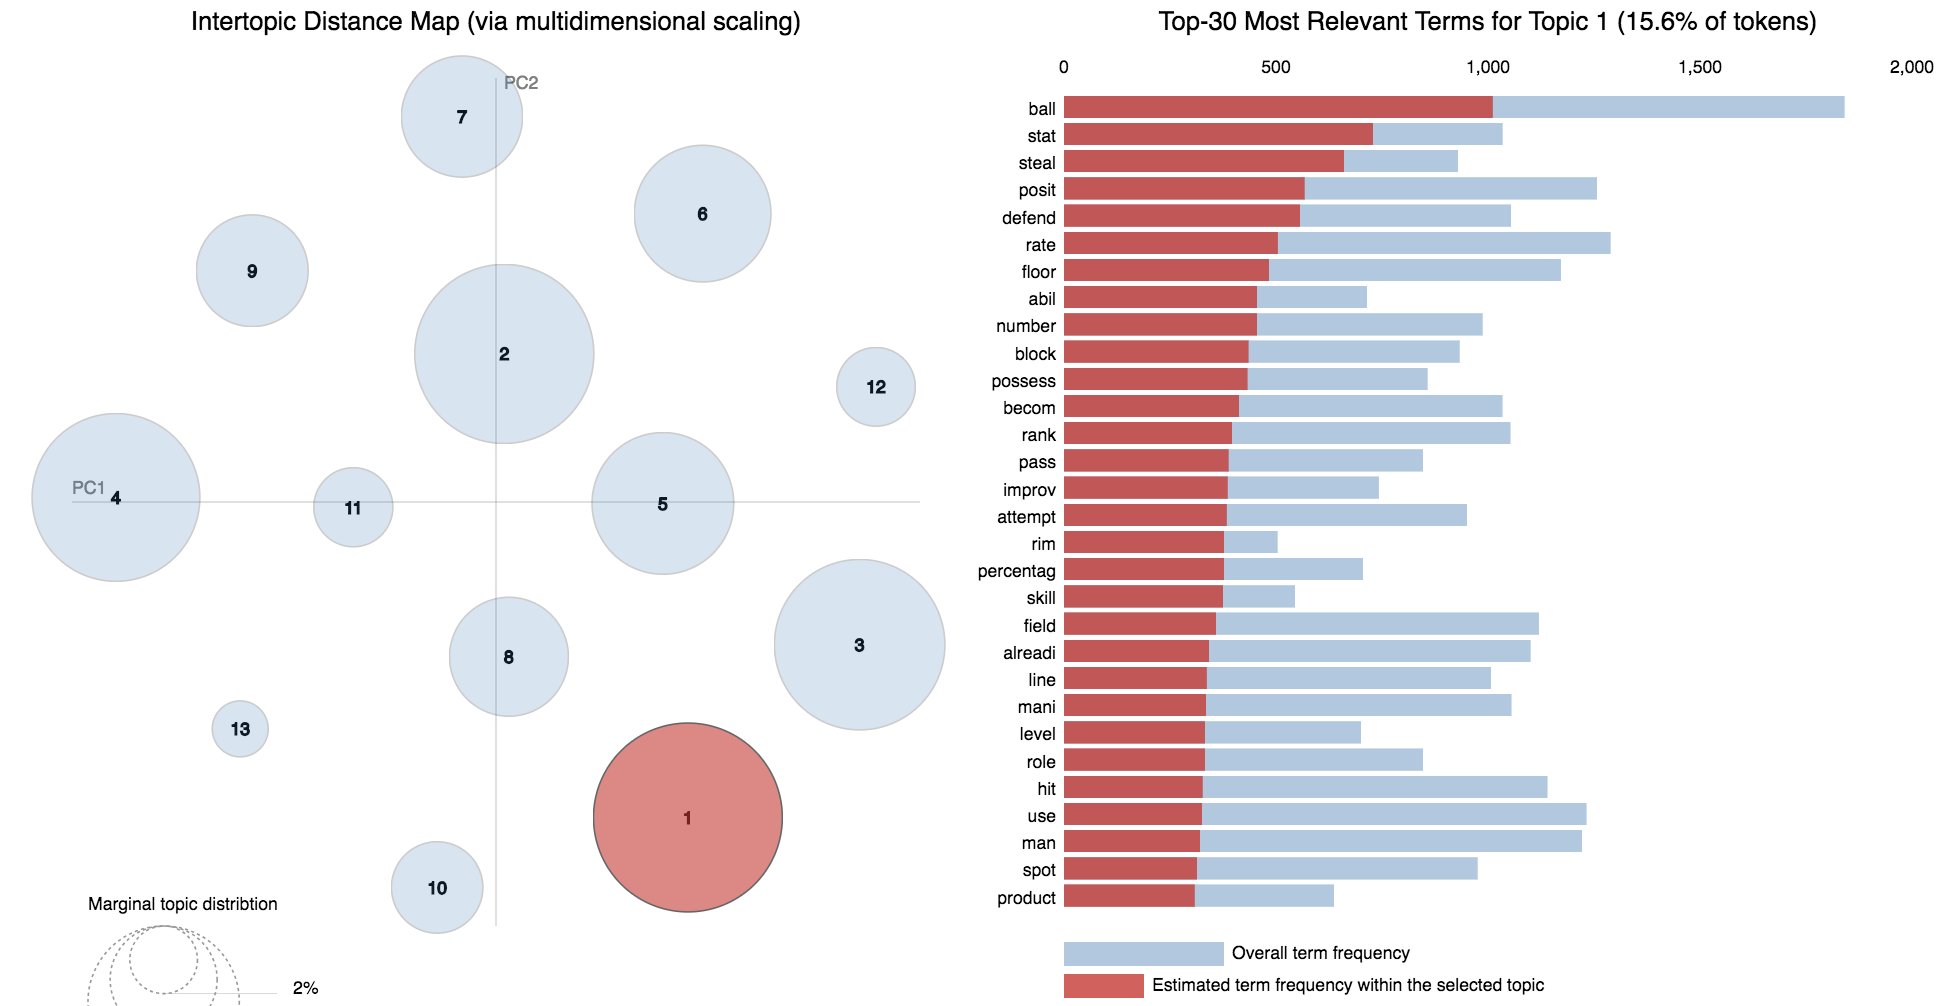
\includegraphics[width=470pt]{1.png} \\

Another large topic, 4, is all about NBA \textit{economics}, including trade deals, free agency signing decisions, and salary information.  In case anyone was wondering, the first four words in this topic tell us a bit about NBA compensation.

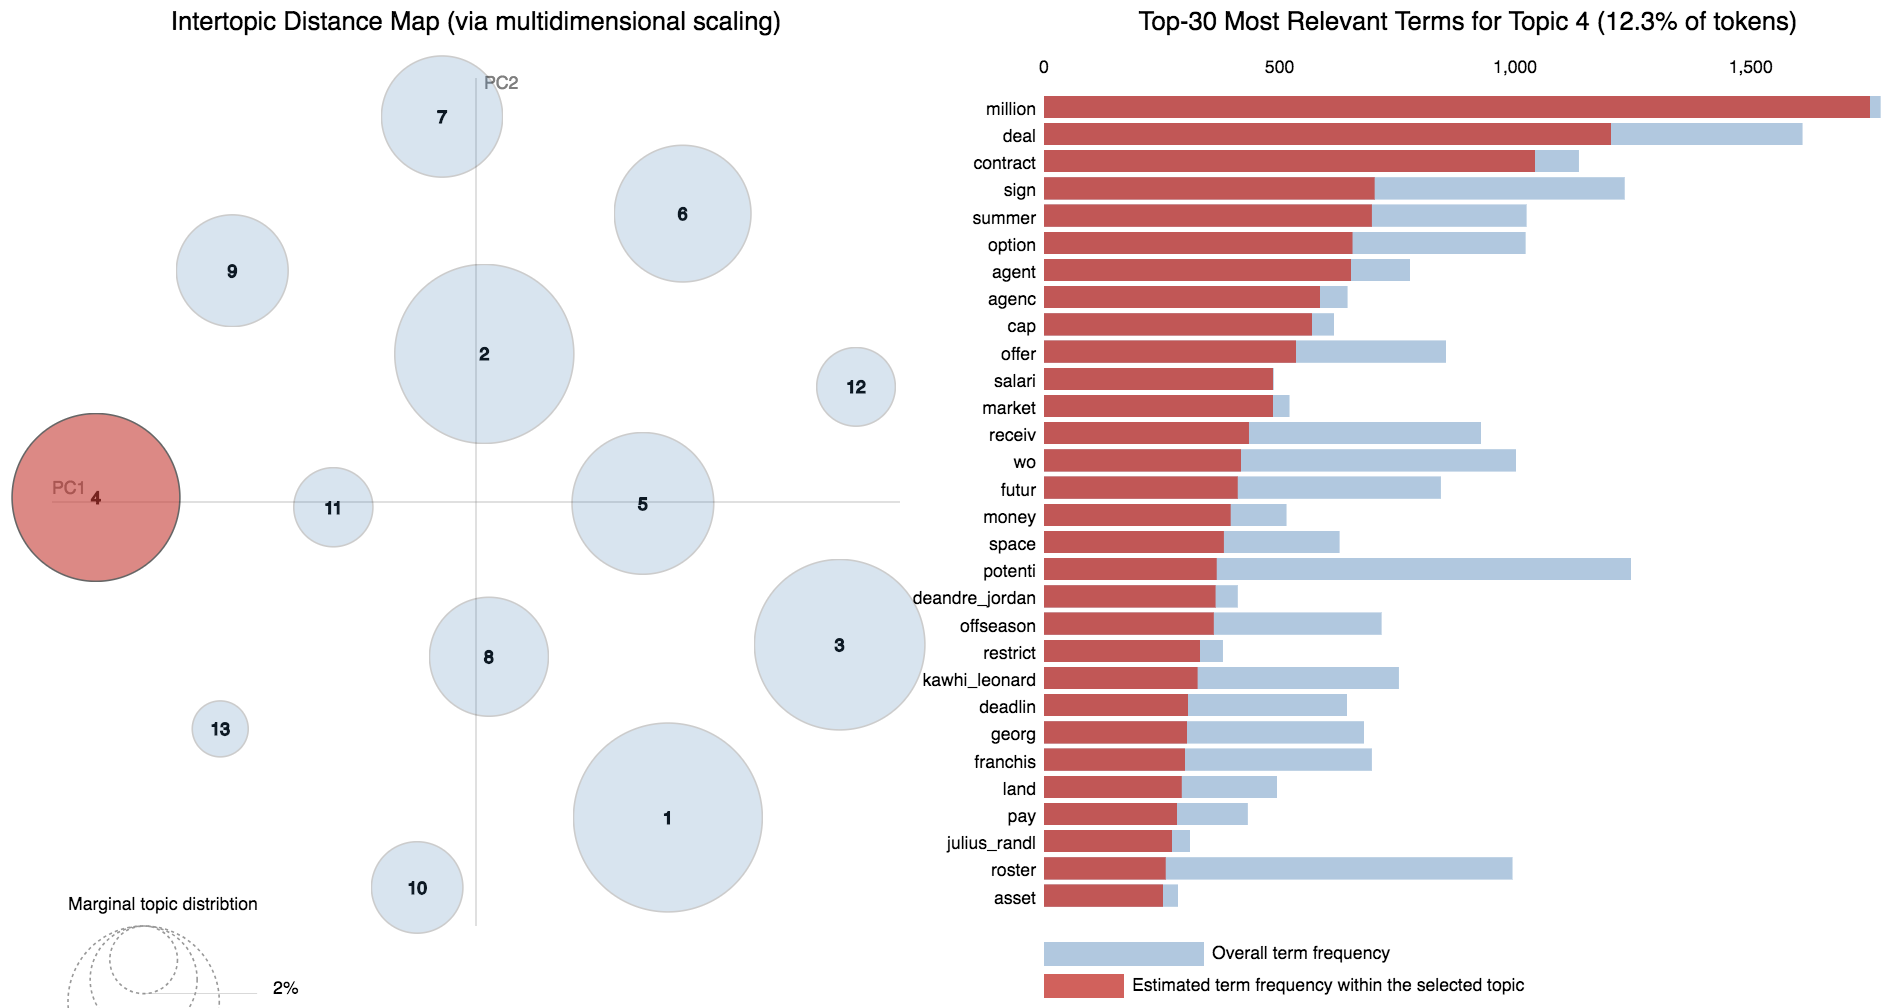
\includegraphics[width=470pt]{4.png} \\

Topic 5, our favorite, is about LeBron James and his team.  The most salient words are LeBron, his team mates, his team name, his coaches, and his major rivals.  

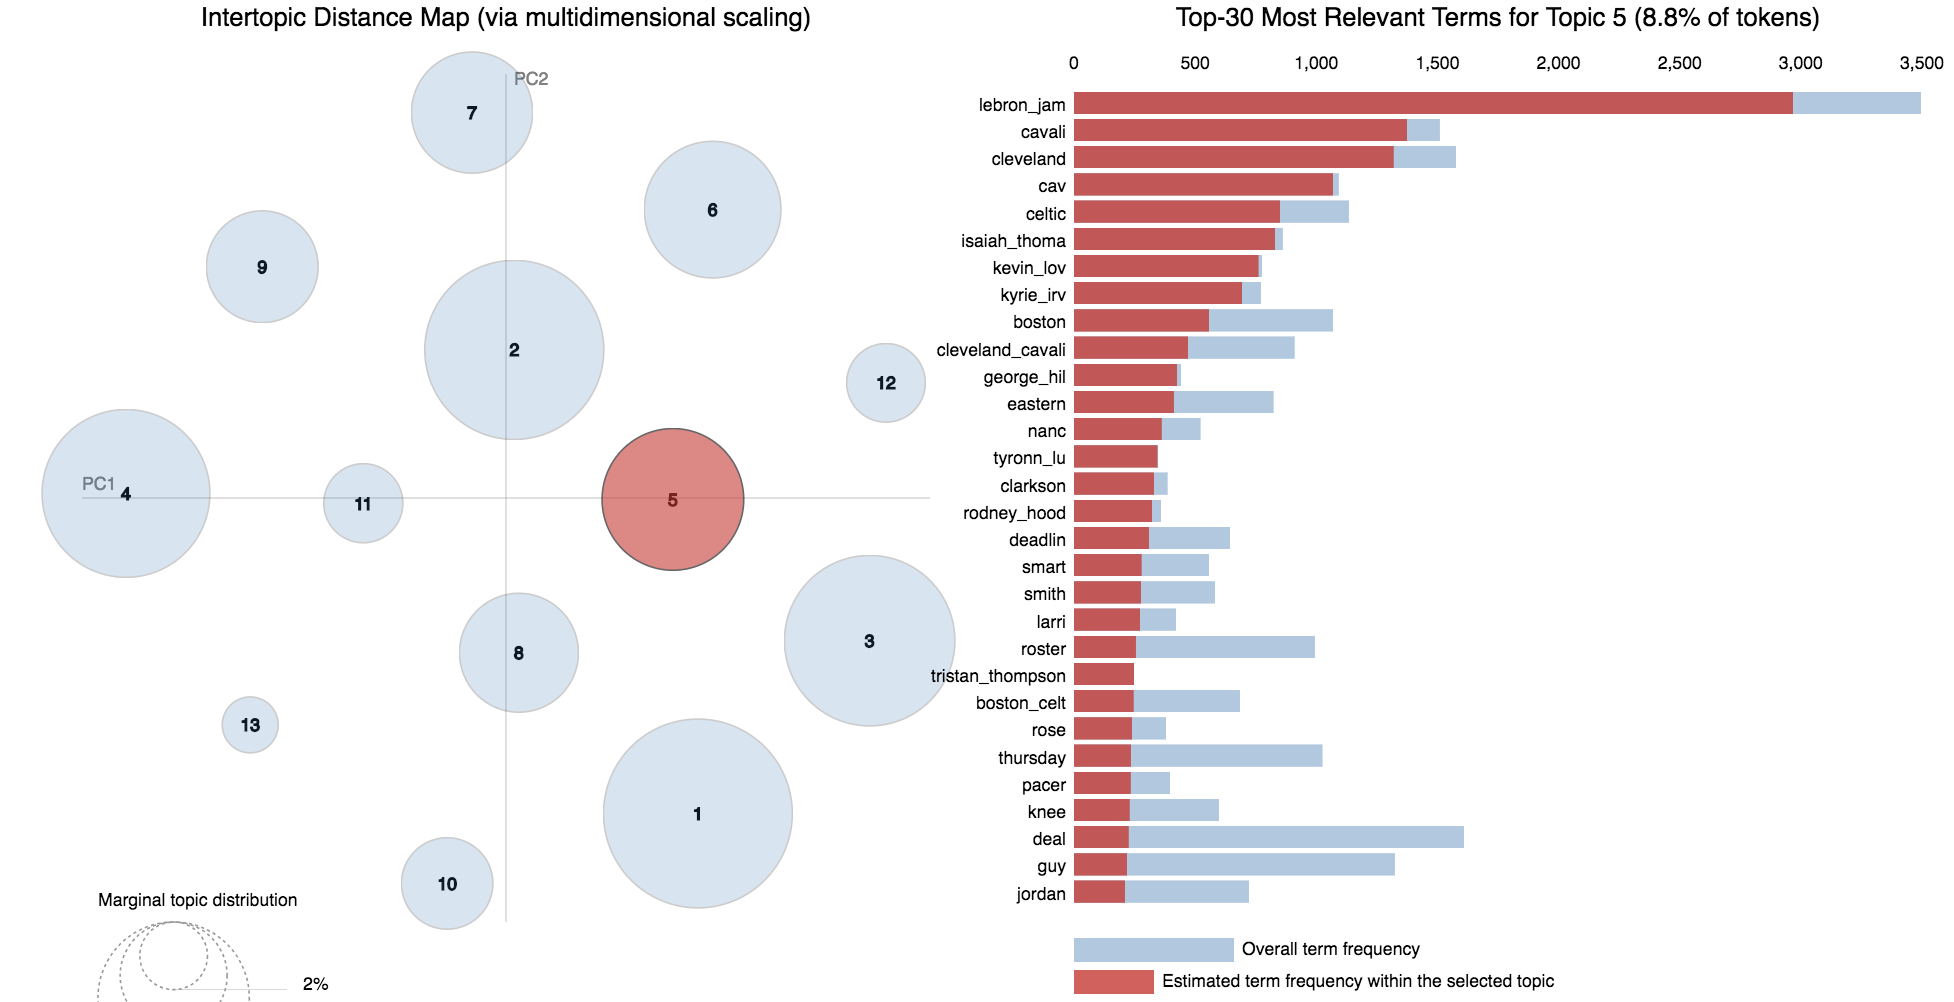
\includegraphics[width=470pt]{5.png} \\

In fact, if you hover over the term \textbf{lebron\_jam}, you can see his primary topics. Topic 5 dominates.

\includegraphics[width=470pt]{5_LeBron.png}  \\

Topic 6 collected the terms pertaining to the NCAA March Madness college tournament, which pushes aside the NBA for a month as college basketball takes center stage.  Michigan and Villanova are primary terms; they played in the championship this year. \\
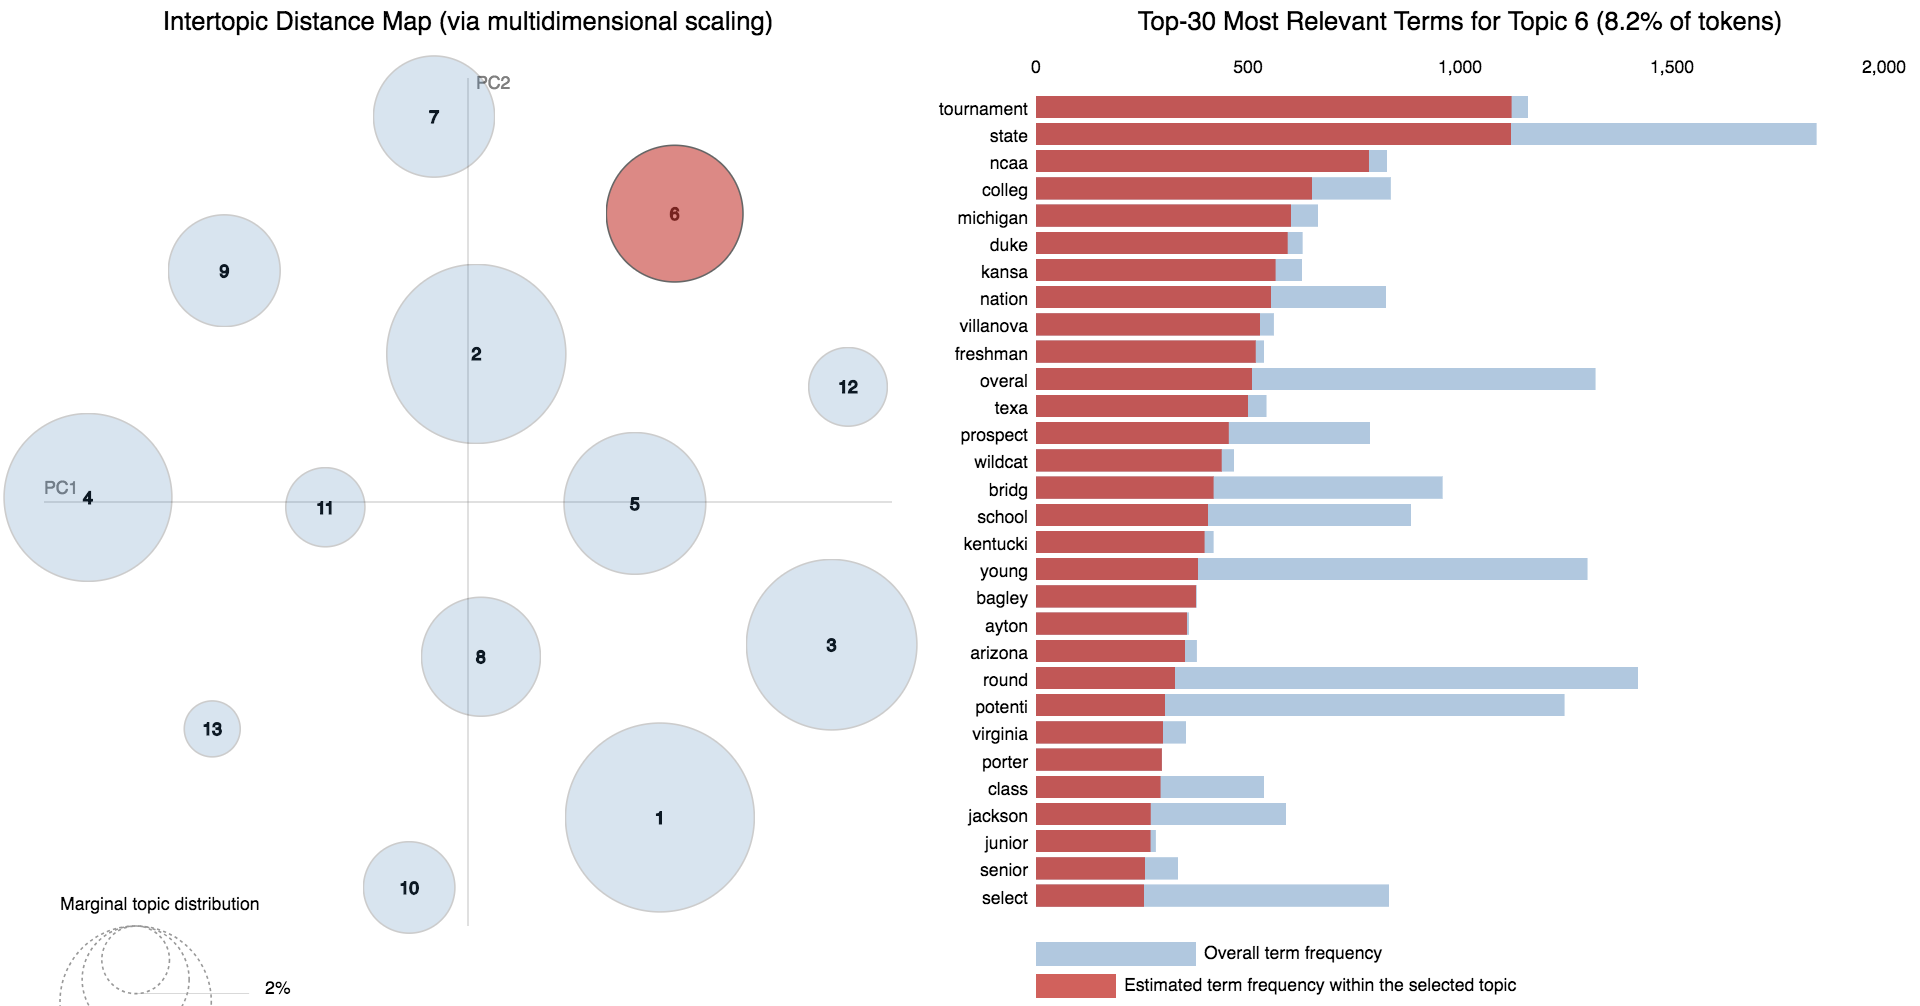
\includegraphics[width=470pt]{6.png} \\s

Topic 13 is actually about soccer!  The API must have returned a handful of soccer-related articles for some reason, and our LDA model discovered that. \\
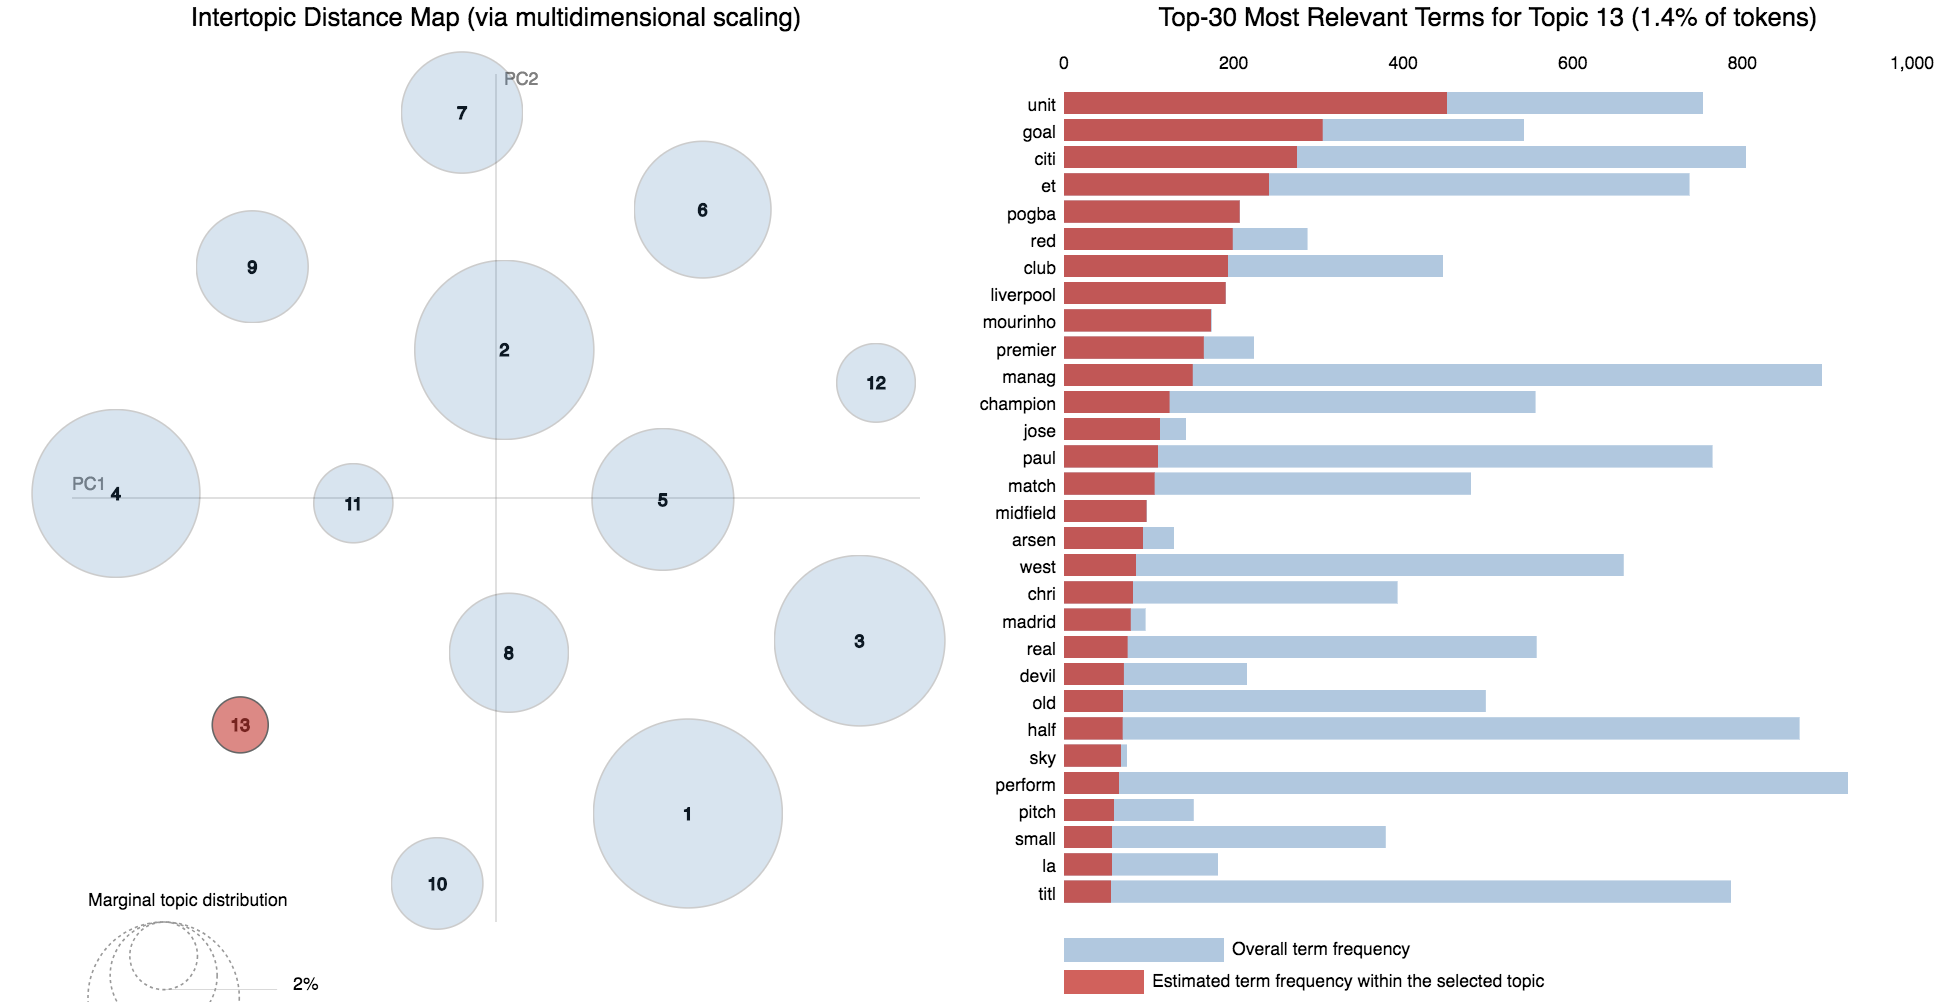
\includegraphics[width=470pt]{13.png} \\

For brevity, we have left other topics in the appendix.

\subsubsection{Sanity Checking the Topics by Clustering Articles by Topical Composition}
The visualizations showed cohesive and comprehensive topics. However, we wanted to cluster the articles in topic space as a final sanity-check.  We used K-Medoids for clustering, since it allowed us to provide a custom distance function. \footnote{KMeans does not necessarily converge for non-Euclidean distances}  Our custom distance function was the Jensen-Shannon divergence metric, which as mentioned above, measures the similarity between two probability distributions.  This distance was appropriate because the articles have been embedded as topic mixtures.  (An alternative method could be to cluster the articles by their most prevalent topic.)  We found $k=8$ to be the number of clusters that captures most of the variation in the articles without overfitting. We found this by plotting the total sum of distances to each medoid for various numbers of medoids, and then looking for the elbow point.  \\

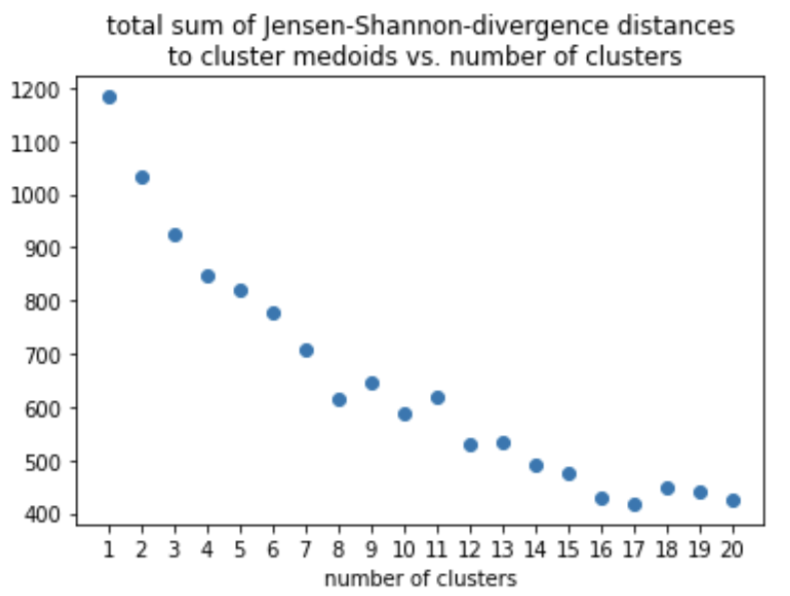
\includegraphics[width=300pt]{jensen.png} \\

Here we plot the two SVD decomposed components for each article, coloring by cluster.

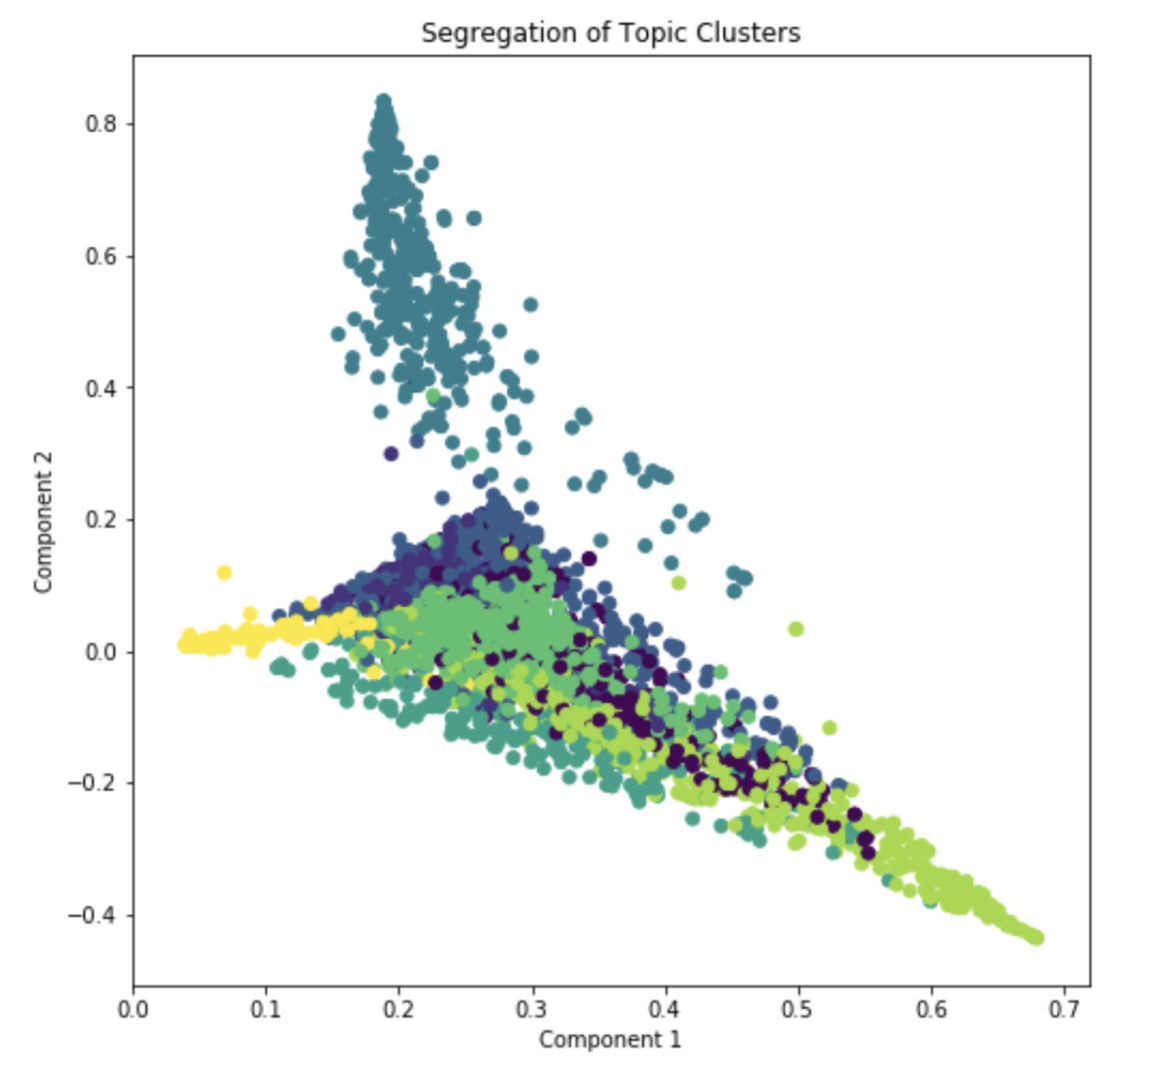
\includegraphics[width=300pt]{svd_clusters.png} \\

The first two components only capture 20\% of the variation in the data, so a 2D visualization drops a lot of information.  But it is interesting that the most distinct cluster (the teal cluster on top) corresponds to articles which are all about \textit{college} basketball as opposed to \textit{NBA} basketball. Here are the 10 titles closest to the medoid of that cluster.  They're all about the March Madness tournament. 

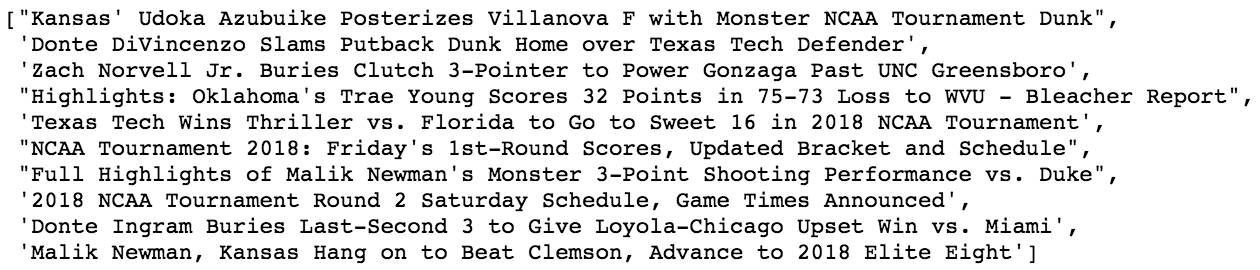
\includegraphics[width=400pt]{college_medoid_closest10.png} 

Across the board, our topic-based clustering seemed to make good sense, so we feel confident in our topics. 

%\section{Producing a Recommendation: An Example}
%Let us see our recommender system in action.  We took a new article from May 13, 2018, entitled \textit{Keith Pompey on 76ers' Pursuit of LeBron James: Prepared to Do Whatever It Takes}, and expressed it as a distribution over the 13 topics using our trained LDA model.  Here is the distribution over topics.  We've labeled each topic according to what we think it primarily represents (as specified above and in the appendix). Not suprsingly, this article is mostly about free agency and trades. Also, notice that the topic of the 76ers is prominent. 

%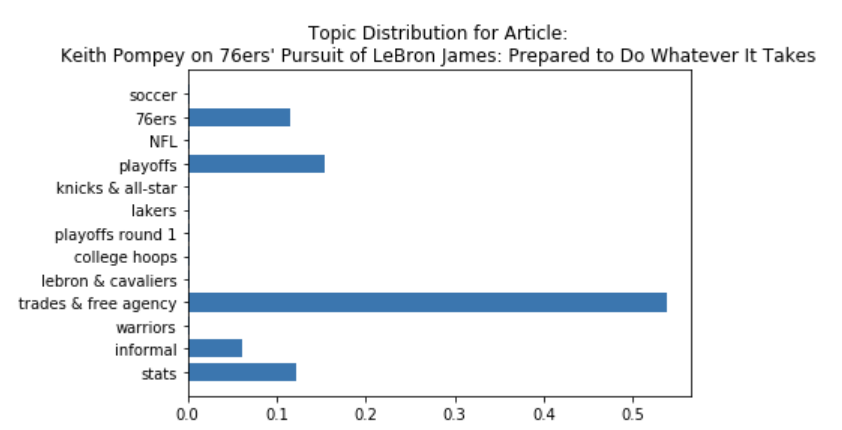
\includegraphics[width=300pt]{newarttopics.png}\\

%MAKE THIS JENSEN SHANNON DISTANCE!!!!!!

%Then, we found the nearest article to it using L2 norm, from all articles in the Bleacher Report corpus expressed in terms of their topic mixtures. Here's are the top 5 recommendations: \\
 
% 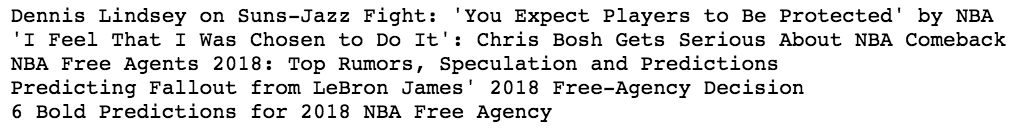
\includegraphics{preds.png}\\
 
% While some articles feel like they are not relevant (notably the first two), notice that the other three recommendations are on-point in discussing LeBron James' upcoming free agency decisions. 

\section{Discussion}
Most of the world's data is unstructured natural language, and NLP provides an analytics edge in many online domains.  In this project we learned a lot, from data scraping and cleaning to building topic models. We explored three common ways of finding vector-embeddings for articles, and then we took a deep dive into one of them, topic modeling with Latent Dirichlet Allocation. The vector-space article embedding was motivated by a desire to provide nearest-neighbor based recommendations.  This project does not test specific recommendations, as it explored only the article-embedding approach.  But an exciting next step would be to test our topic-based recommender system using click-through data from BleacherReport.com.

\newpage

\section{Appendix}
\subsection{Initial Experiment to Find Most Promising Model}
\subsubsection{Word2vec}
Word2vec is a modeling approach that aims to embed words as vectors by considering their context in a corpus.  In a successful model, words that share common contexts correspond to vectors in close proximity in the space.  In our case, we with to embed \textit{articles}, not words,  so the approach we tested was to \textit{average the word embeddings in the title of the article}. 
%\subsubsection{Word2vec Pre-processing}
Word2vec training requires a set of sentences, not documents, so we began a different data-processing pipeline just for this model, starting from the scraped documents. In addition, we left in all of the words, as opposed to removing them as in the other models. The reason for this is that word2vec infers dependency information between words, and removing stop words would remove that linkage information.
%\subsubsection{Word2vec Training}
The number of word2vec dimensions is a hyperparameter that depends on the application. Most literature recommends a value of 100, and this produced very reasonable results in our case.

The closest vectors to lebron\_james are his (all-star) teammates, his hometown, his team name, his trash-talking nemesis and other all-star rivals. \\
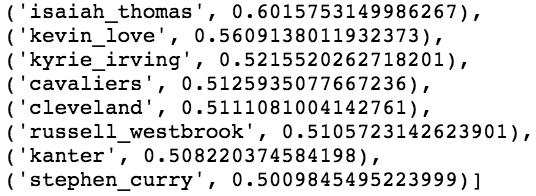
\includegraphics[width=200pt]{james_word2vec.png} 

The model correctly separates teams from the Eastern Conference from teams in the Western Conference, which you would expect from a Bleacher Report corpus with many articles about each conference separately. The model also places team mates in close proximity and can differentiate between teammates and non teammates. \\
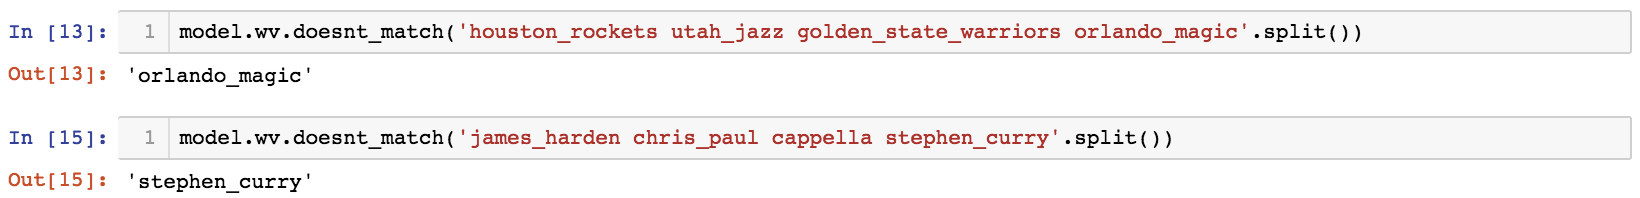
\includegraphics[width=450pt]{word2vec_diffs.png} 

\subsubsection{Non-Negative Matrix Factorization}

Non-negative matrix factorization is a group of algorithms with a strong application in recommender
systems. In our case, we will use NMF to find the underlying topics in our corpus. The mathematical
basis of NMF is quite different from LDA: basically, LDA is based on probabilistic graphical modeling
while NMF relies on linear algebra. Thus, we were curious to see which would perform better on
our corpus.

\subsubsection{Experimental Results: LDA Wins}
We applied both NMF and LDA to our corpus and eye-checked the results. At this point, our goal
was just to see if NMF would perform better than LDA, in order to choose which method to
continue with. We already found interesting packages to visualize LDA results, so
LDA was our first choice but we still wanted to check if NMF would be more suited,
though we acknowledge eye-checking might not be the most rigorous approach.
We chose to return $k=10, 13, 15, 17, 20$ topics and printed the top 10 words for each topic.
Overall, LDA returned more consistent results, while NMF would regularly return topics that 
we cannot clearly label. For example, how would we label topic 1 in the following results:

\begin{ttfamily}
 Topic 0: points game rebounds series rockets season jazz thunder games assists\\
Topic 1: nba mj triple 30 way best liangelo possiblethe clowning doublesthe\\
Topic 2: draft nfl browns lb landry app football wnba journey st\\
Topic 3: ...
\end{ttfamily}

We proceeded similarly for word2vec and concluded we should stick to LDA.

\subsection{Topic Modeling and LDA Background}
In topic modeling, we attempt to discover $k$ \textit{topics} from among our article, and to identify the proportion of each topic in each article.  A \textit{topic} is defined as a frequency distribution over all words in the vocabulary; for each topic, each word has a frequency of occurrance.  If topic modeling is successful, the high-frequency words for each topic will frequently appear together in text and will resemble the human understanding of a topic. 

Let \\
$D = \{d_1, d_2, ... d_N \}, \quad$ the set of $N$ documents (articles) obtained from Bleacher Report \\
$V = \{w_1, w_2, ... w_M \}, \quad$ the set of $M$ words in the final vocabulary \\
$T = \{t_1, t_2, ..., t_K\}, \quad$ the set of $K$ topics in the documents 

LDA is a bag-of-words model, as opposed to one that considers grammar.  It assumes that each document is created according to the following generative process: \\
$\text{} \quad$ 1. Randomly generate a distribution over topics\footnote{This requires a distribution over a distribution. The  topic distribution is assumed to have a Dirichlet prior, giving the model its name}. \\
$\text{} \quad$ 2. To come up with each word in the document: \\
$\text{} \quad$ $\quad$ a. Randomly choose a topic. \\
$\text{} \quad$ $\quad$ b. Randomly choose a word from that topic. 

As mentioned above, the method's name comes from the sparse Dirichlet priors that the model employs: the assumption is that each document is composed of only a small set of topics, and that each topic primarily covers a small set of words.

We provide $k$, the number of topics, and then the task of LDA is to infer the following two parameters, by maximizing the likelihood (according to the story of the generative process described above) of the articles in our corpus: \\
$\text{} \quad \beta_t$: the distribution over words for topic $t$: $\mathcal{P}(w | t) \quad \forall w \in V$ \\
$\text{} \quad \theta_{dt}$: the proportion of document $d$ that came from topic $t$: $\mathcal{P}(t | d) \quad \forall t \in T$ 

\subsection{LDA Visualization Continued}
Topic 3 seems to be about the Golden State Warriors, the best team in the NBA (mostly because of superstars Stephen Curry and Kevin Durant), and their competition in the Western Conference.

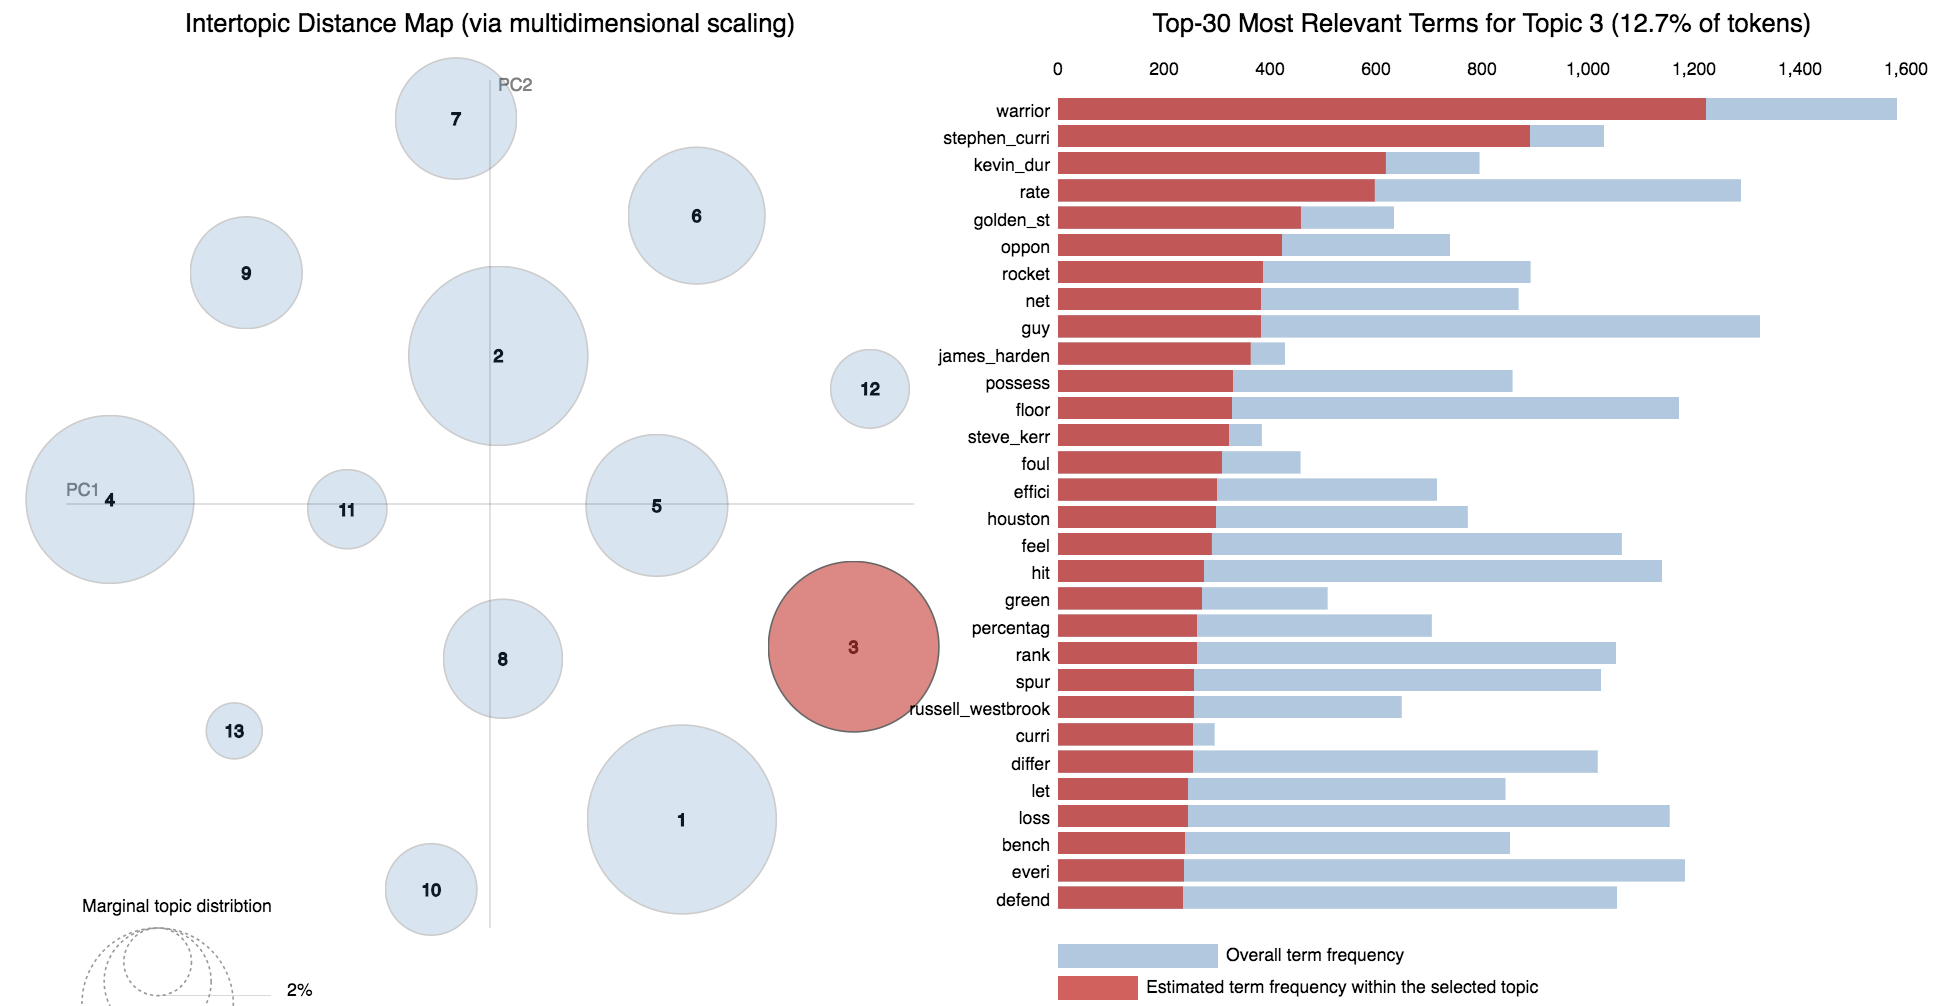
\includegraphics[width=470pt]{3.png} \\

Topic 7 seems to be about the playoffs, seeding, and exciting first-round matchups.  \\
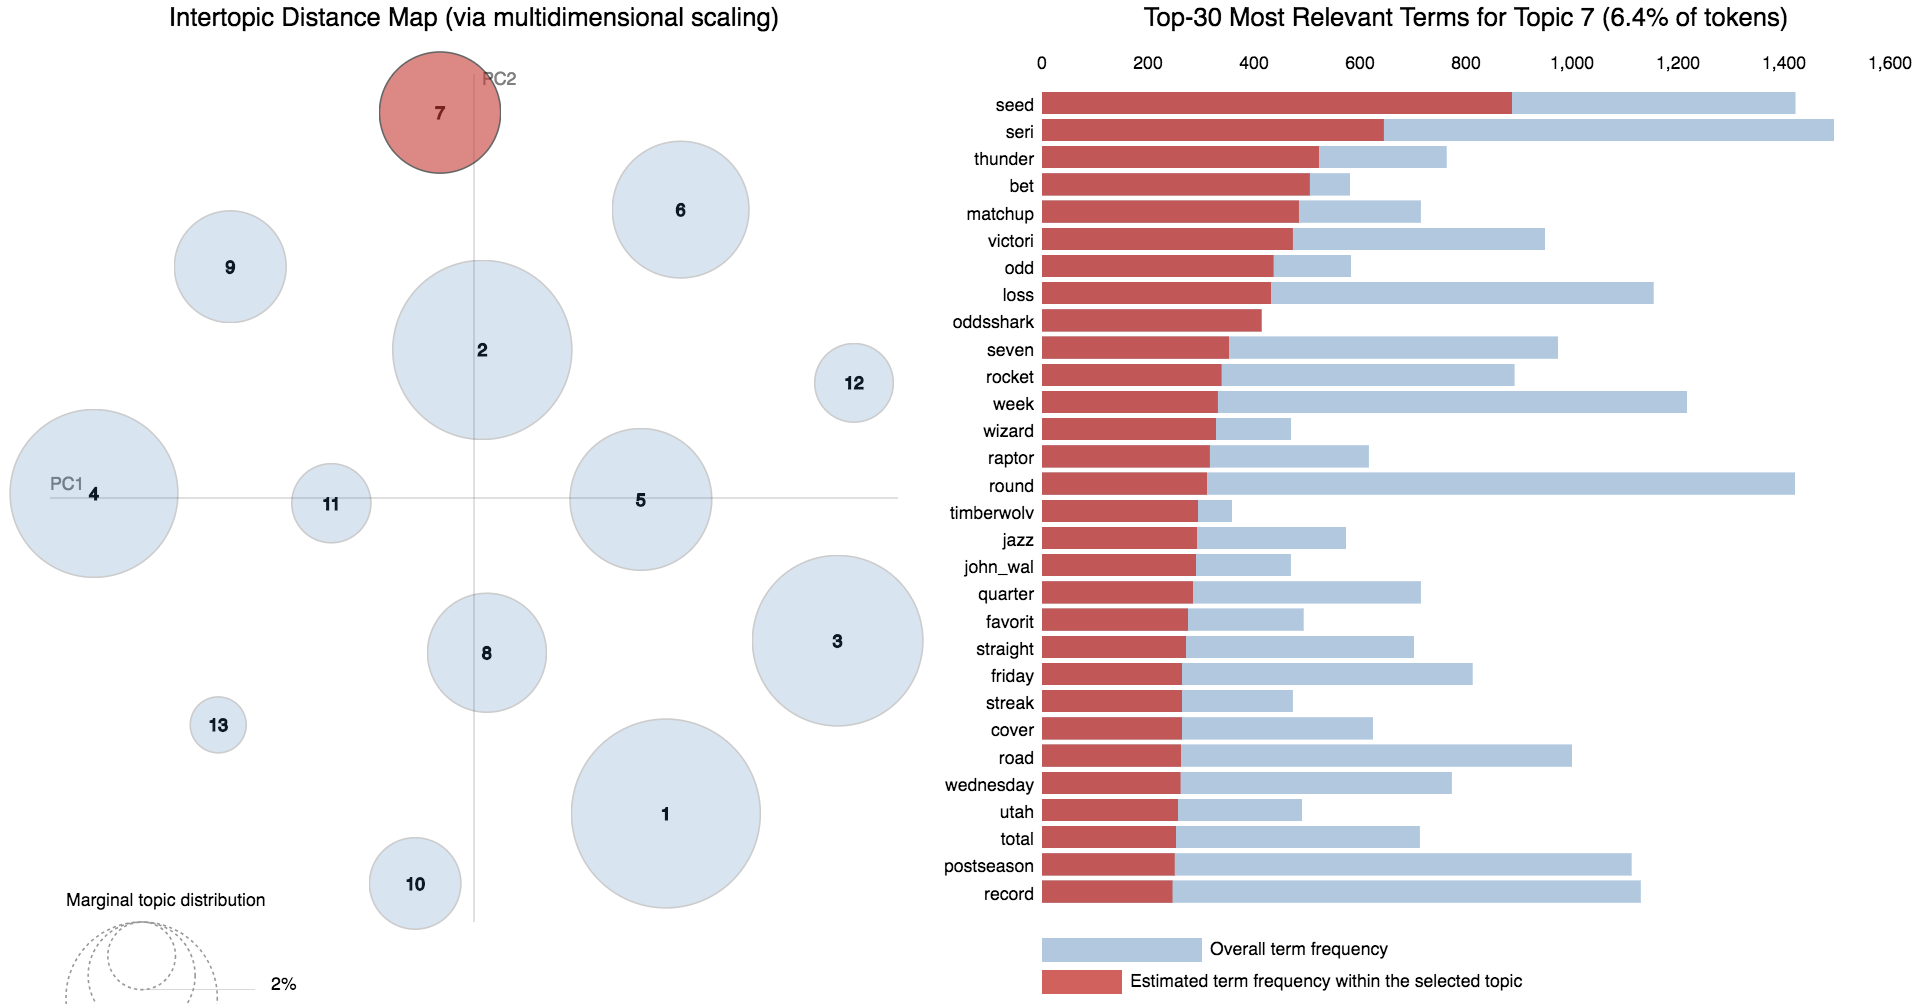
\includegraphics[width=470pt]{7.png} \\

Topic 8 seems to capture the multiple stories around the Los Angeles Lakers this season, always a popular NBA team. 

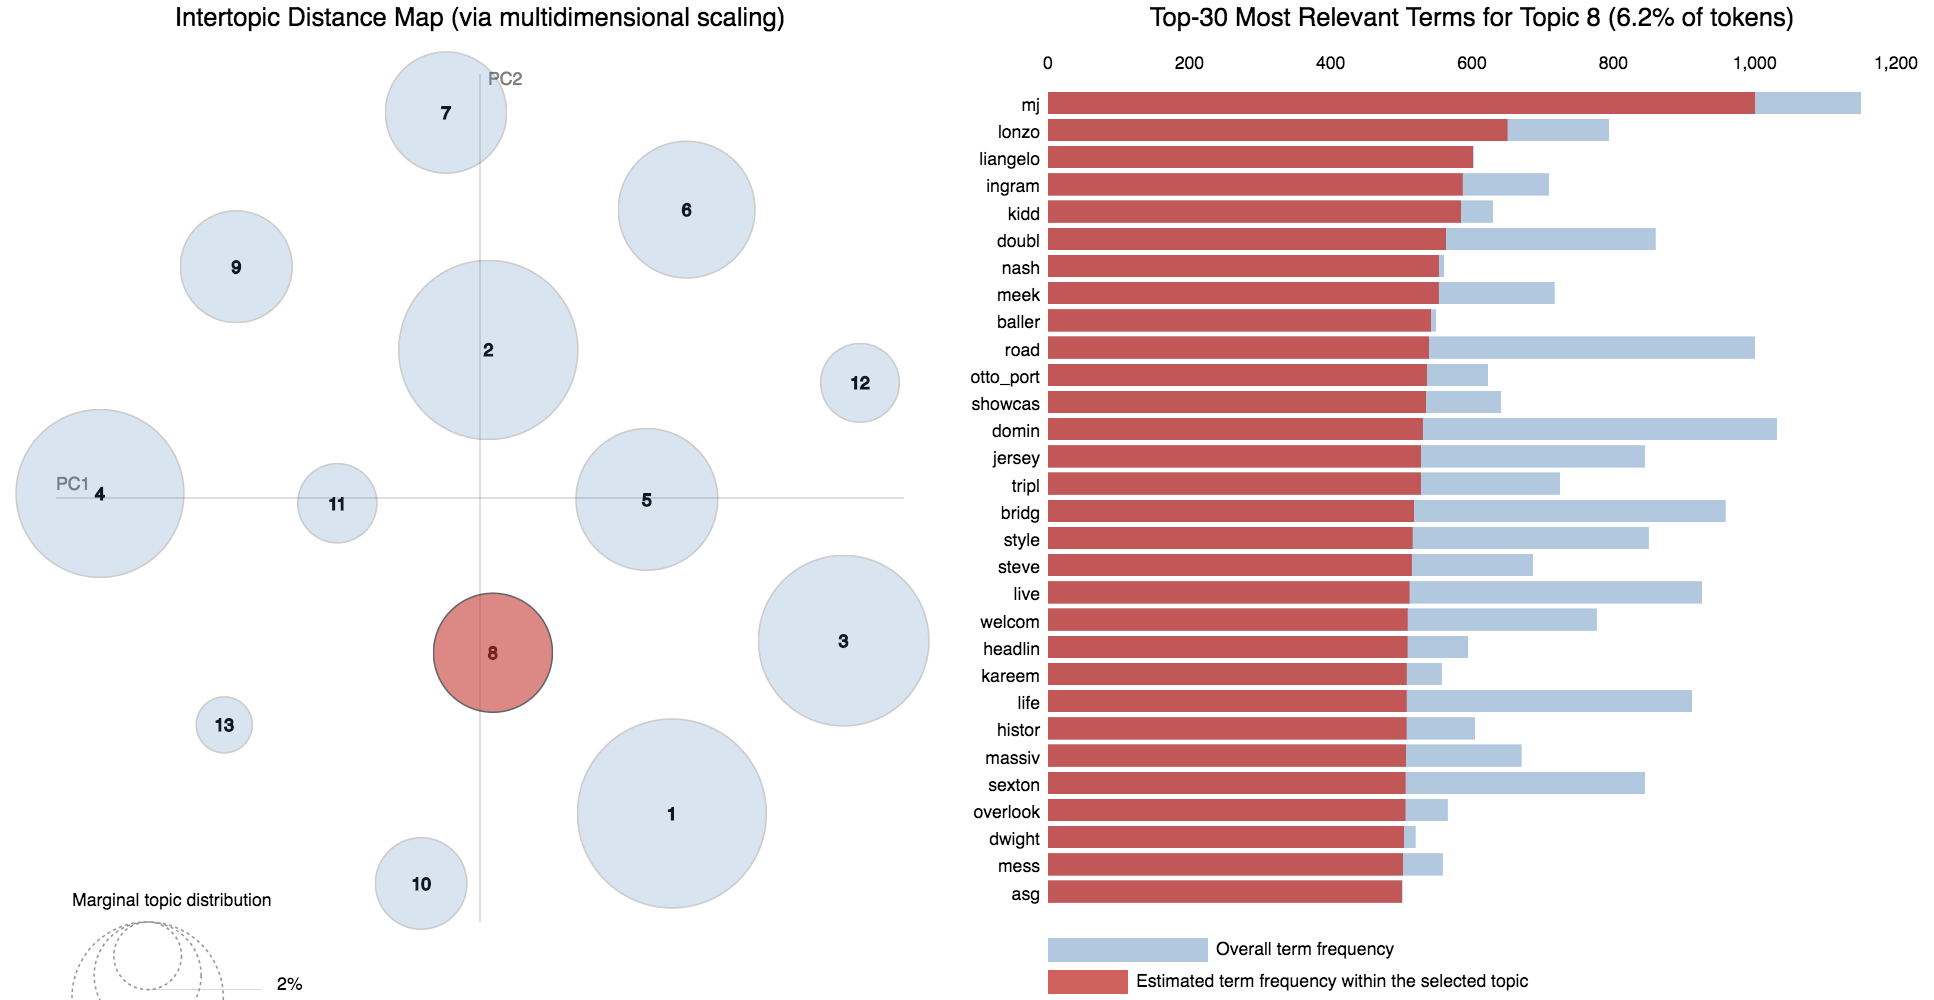
\includegraphics[width=470pt]{8.png} 

Topic 9 seems to merge two distinct topics, in our opinion - the all-star game and the New York Knicks. 

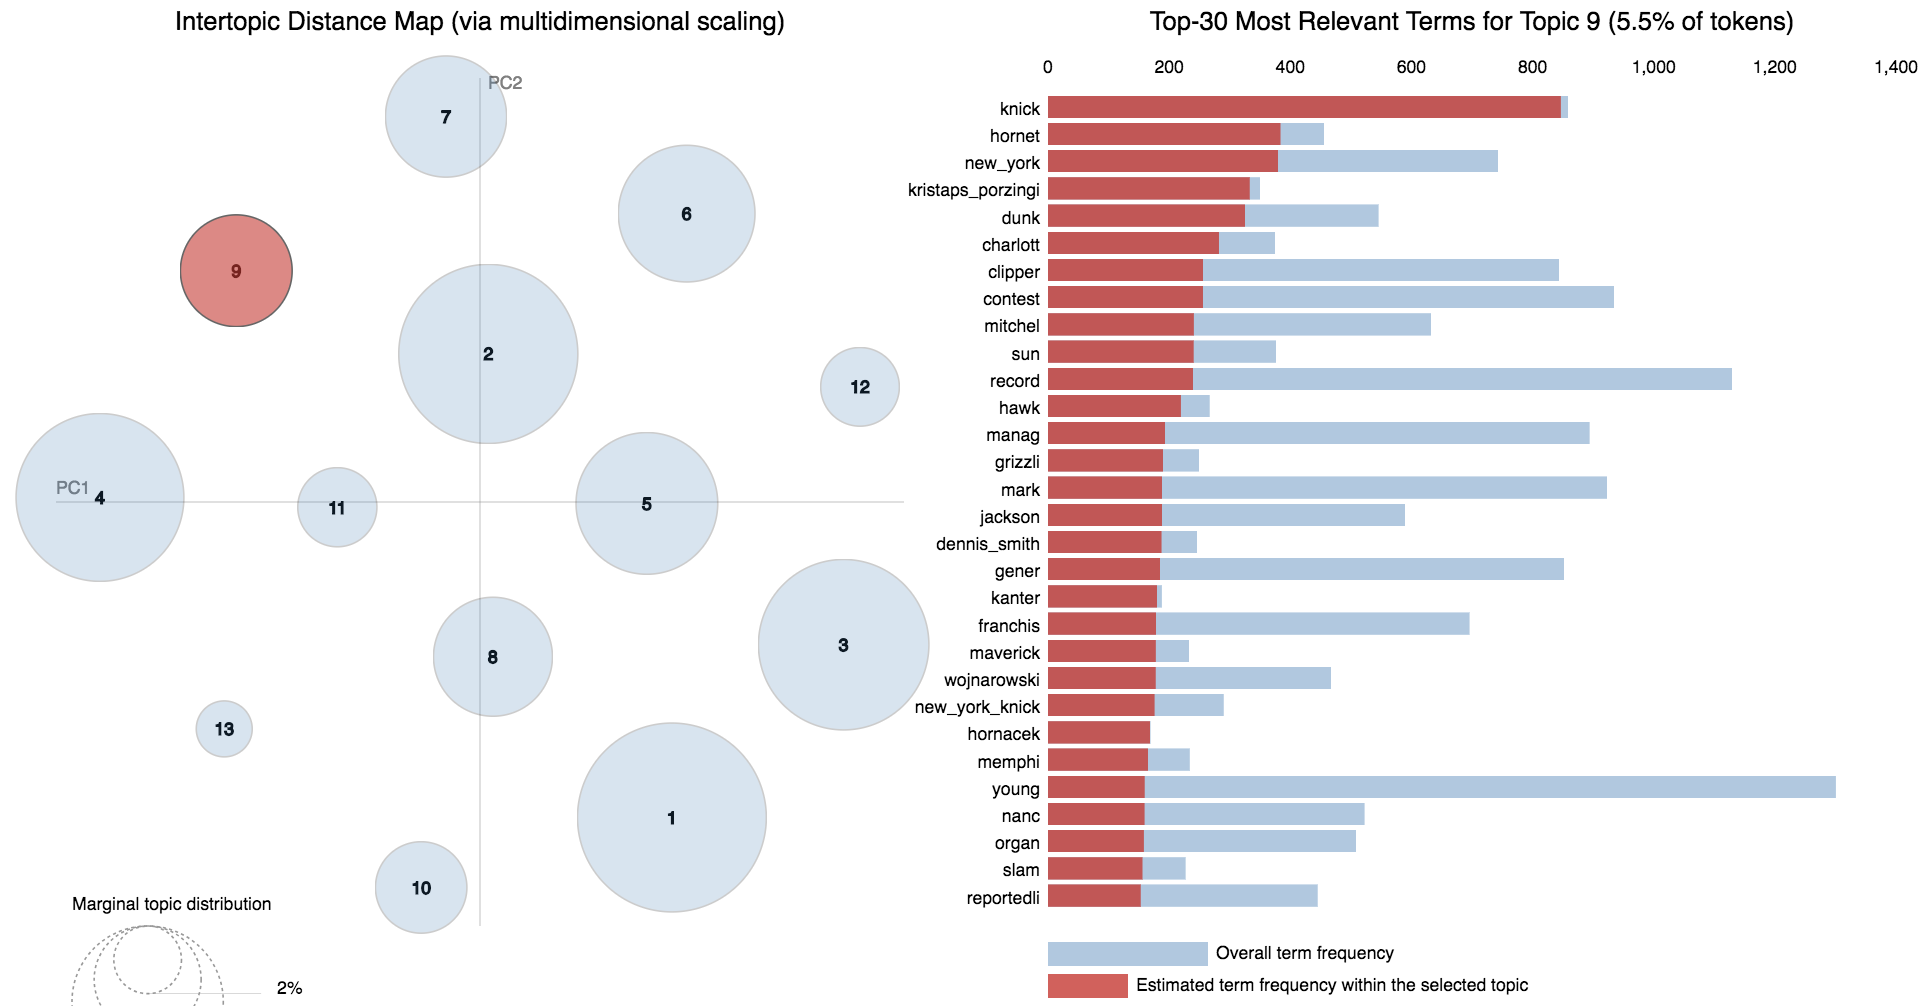
\includegraphics[width=470pt]{9.png} 

Topic 10 is about the playoffs, and includes the most notable postseason teams. 

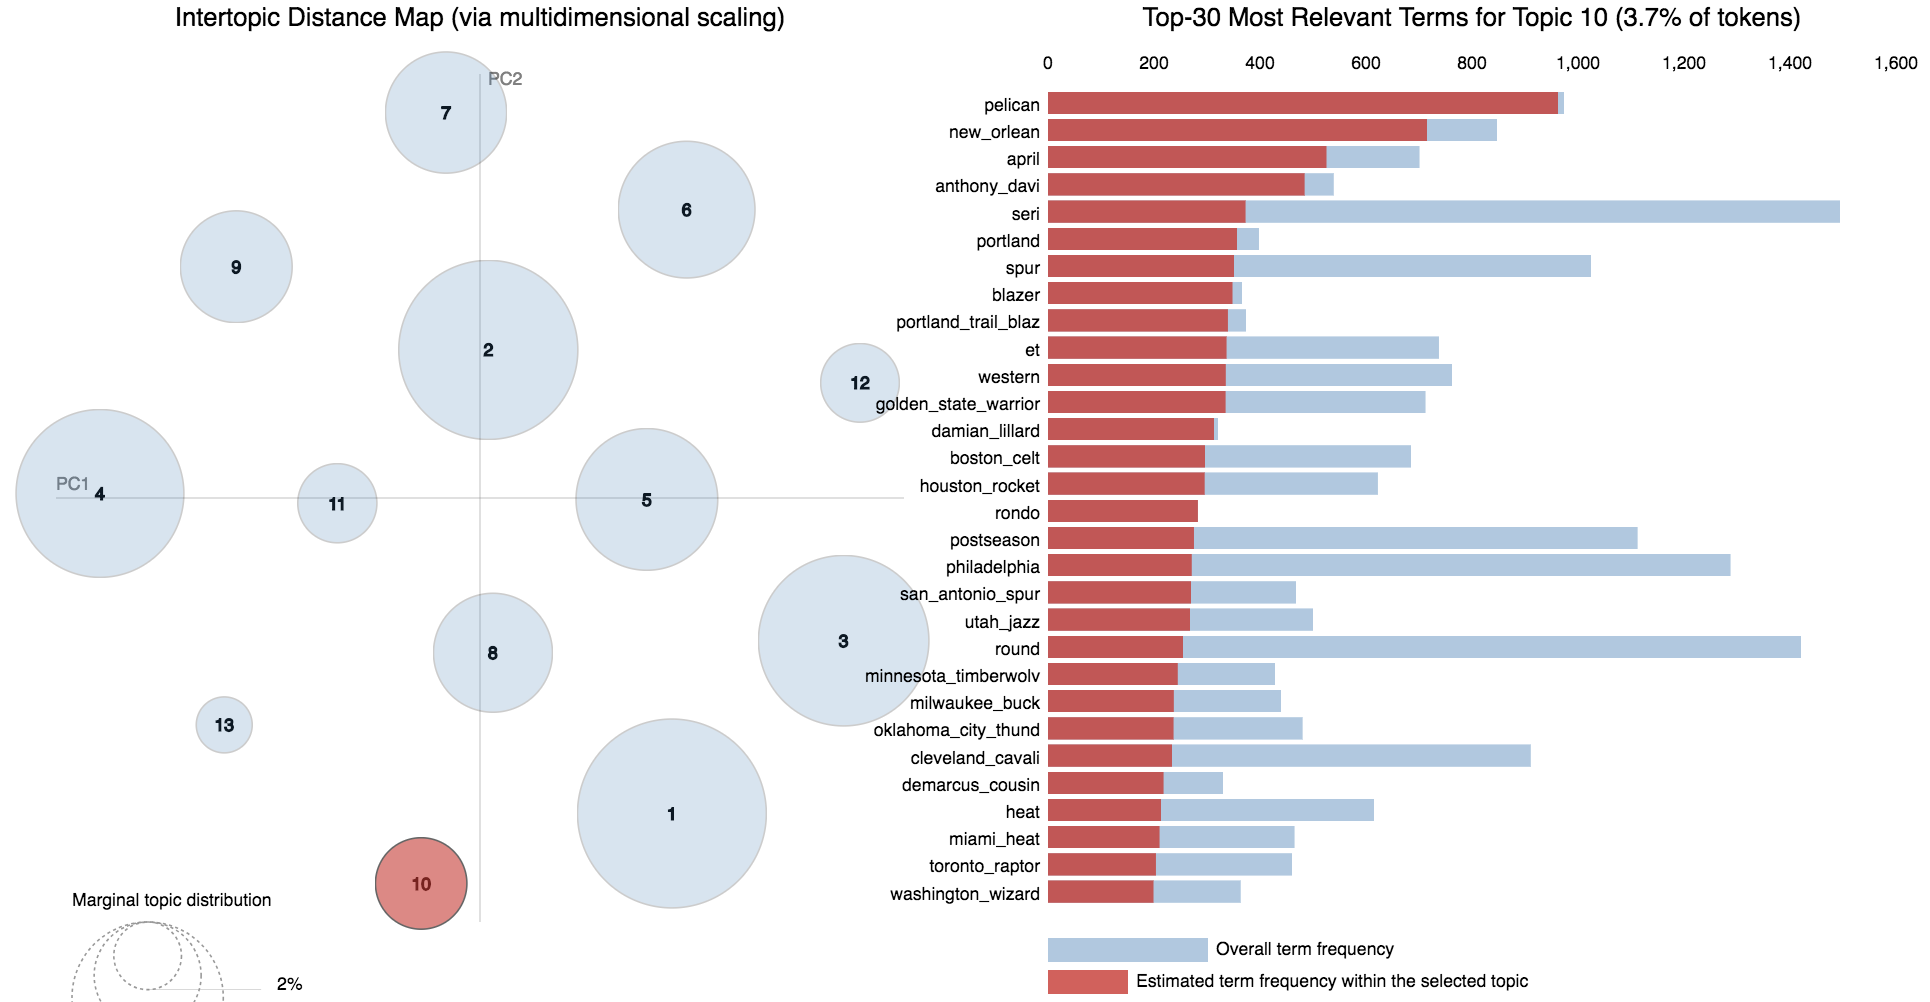
\includegraphics[width=470pt]{10.png} 

Topic 11 is actually about the National Football League!  The NewsAPI must have returned a handful of football related articles with the basketball ones, and our LDA model discovered that. 

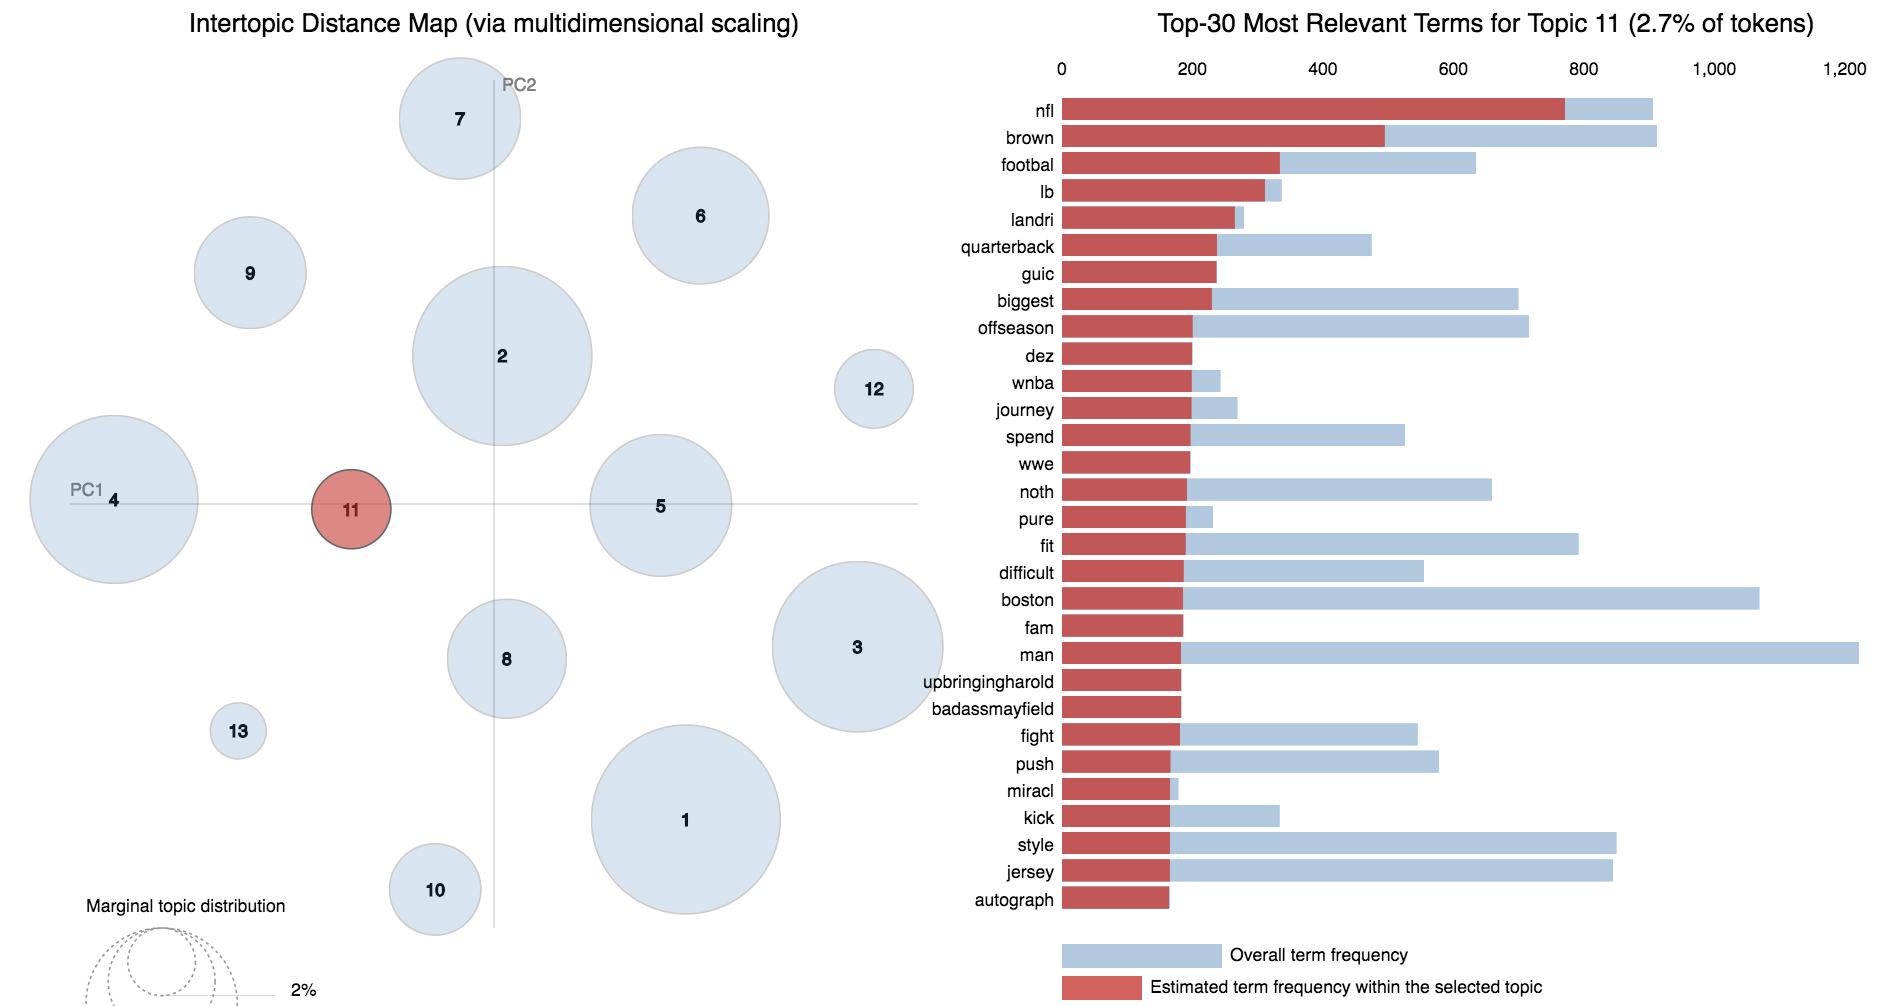
\includegraphics[width=470pt]{11.png} 

Topic 12 seems to be about the Philadelphia 76ers and their rivalry with the Miami Heat this season. The 76ers have been one of this seasons biggest sub-stories because they have two budding young superstars and are seeking to land LeBron James during free agency this summer.

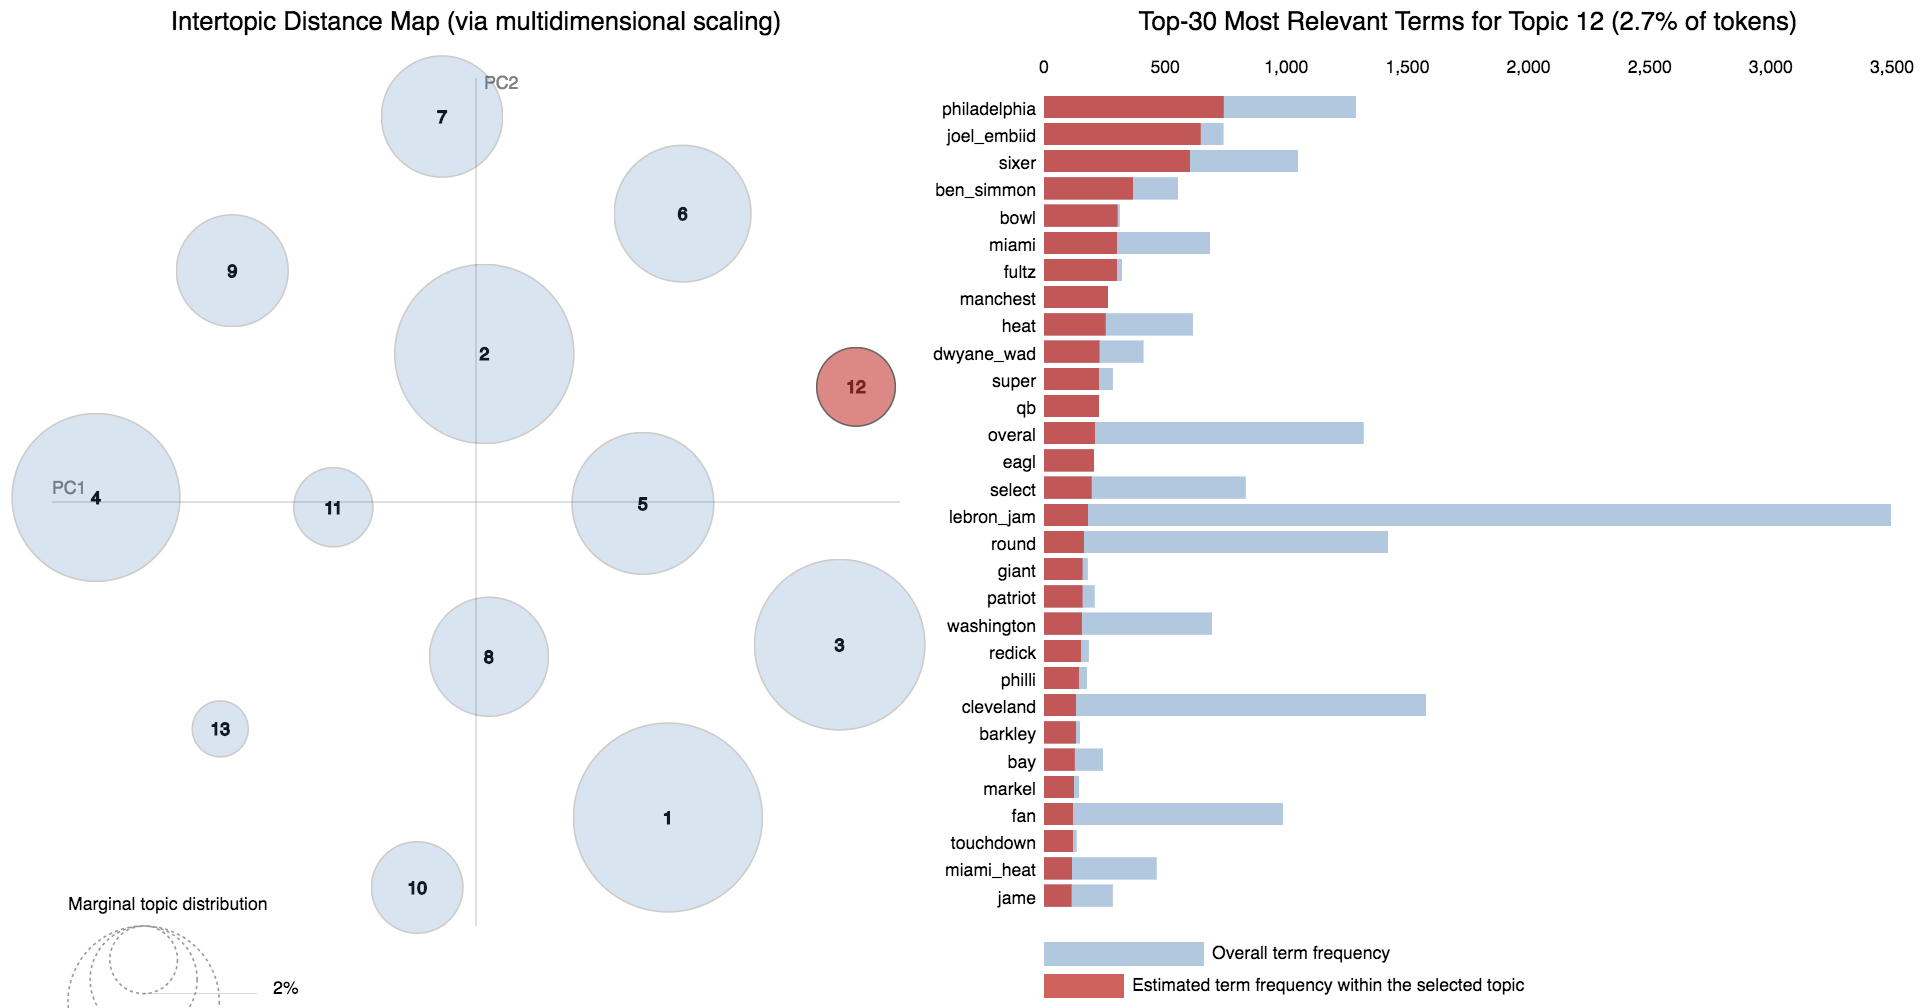
\includegraphics[width=470pt]{12.png} 

Topic 2, located in the middle of the topic clusters, seems to capture informal language. 

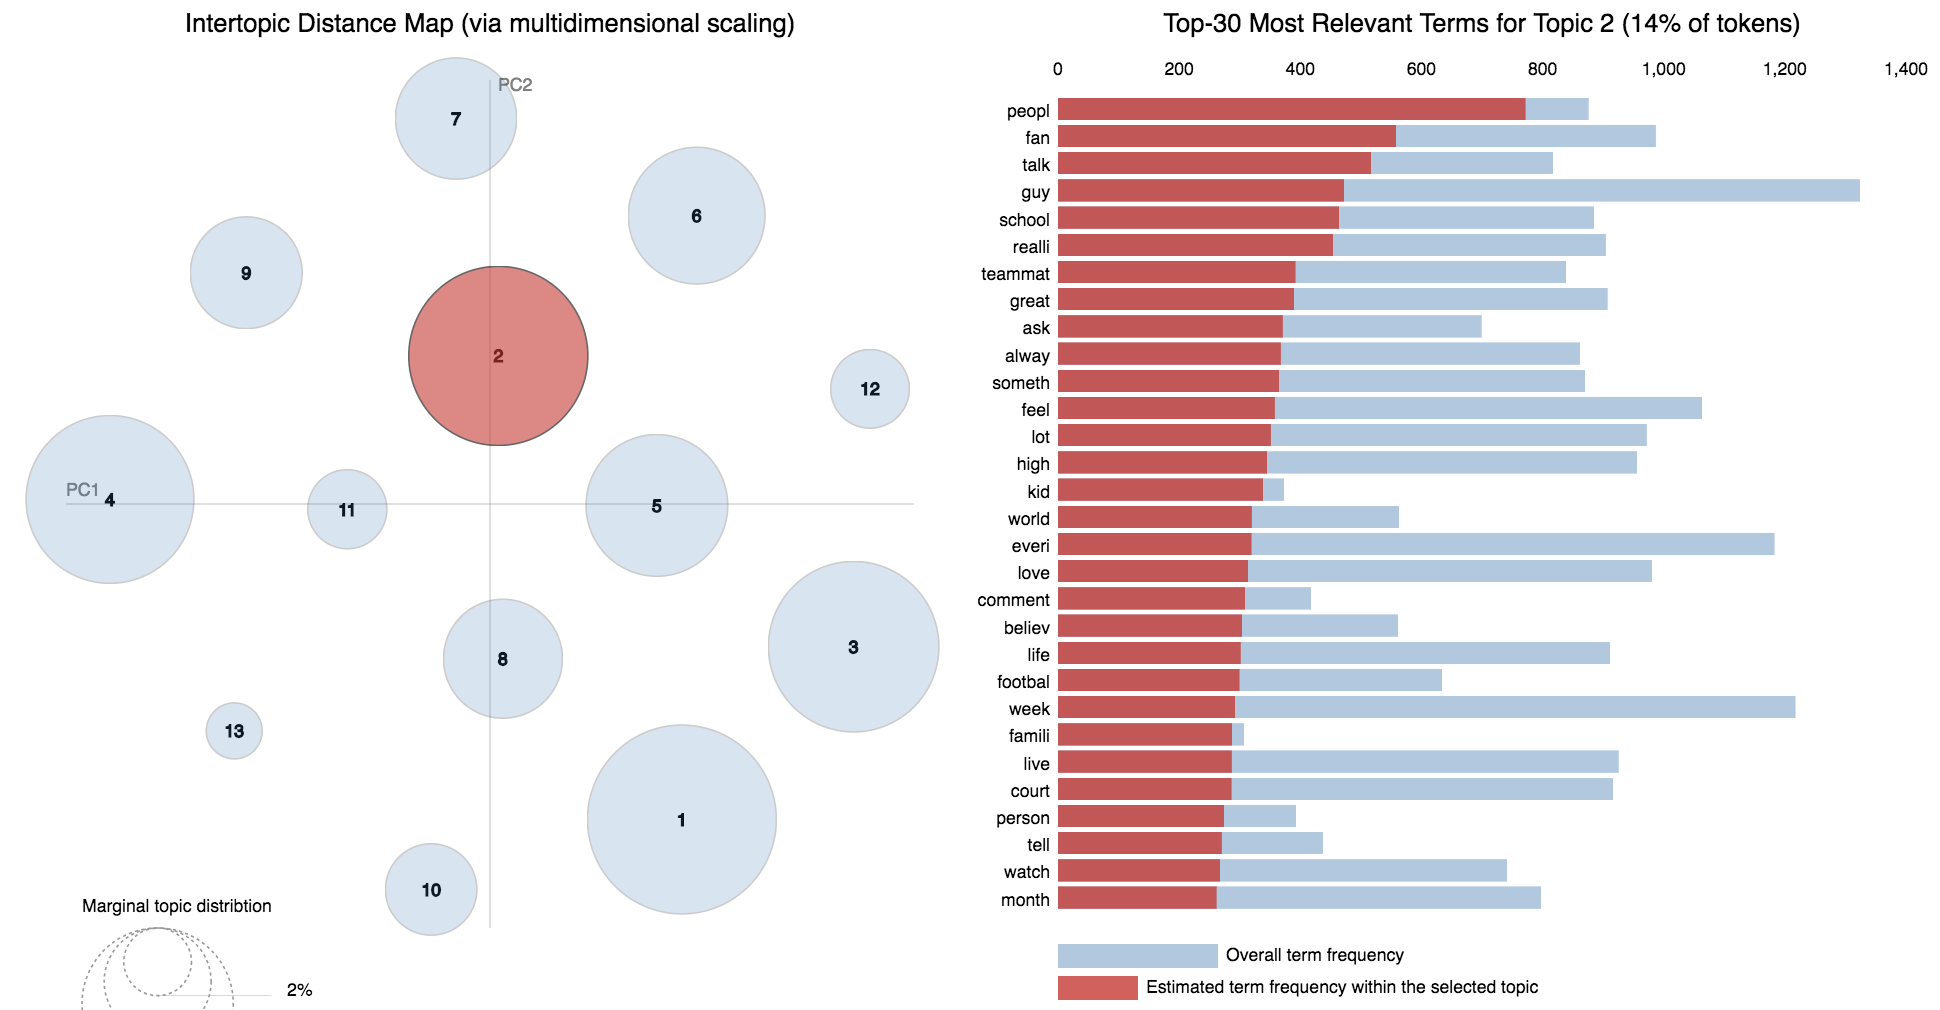
\includegraphics[width=470pt]{2.png} 

\subsection{Code}
All of our code and data can be found at https://github.com/salbro/ae_project.  Many files are now obsolete. If you are interested in understanding our code, we recommend primarily browsing the following files: \\
utils.py: miscellaneous functions that we wrote for cleaning
SA_API_playground.ipynb: Querying the NewsAPI for URLs, and then scraping those URLs to get article content. \\
spa_lda.ipynb and spa_lda_lemmatizing.ipynb: LDA work
lda_nmf.ipynb: NMF work
spa_word2vec.ipynb: word2vec work
spa_clustering.ipynb: clustering documents by topic makeup


our word2vec work
our clustering work

 
%ngram overfitting


\end{document}